\documentclass[11pt,a4paper]{article}
\usepackage[margin=2cm]{geometry}
\usepackage{lmodern}
\usepackage[T1]{fontenc}
\usepackage{amsmath,amssymb}
\usepackage{booktabs,array,tabularx,xltabular}
\usepackage{enumitem}
\usepackage{xcolor}
\usepackage[most]{tcolorbox}
\usepackage{titlesec}
\usepackage{graphicx}
\usepackage{float}
\usepackage[font=small,labelfont={bf,color=headblue},skip=4pt]{caption}
\usepackage[colorlinks=true,linkcolor=headblue,urlcolor=blue!50!black]{hyperref}

\definecolor{headblue}{RGB}{38,70,120}
\titleformat{\section}{\Large\bfseries\color{headblue}}{\thesection}{0.8em}{}[{\color{black}\titlerule}]
\titleformat{\subsection}{\large\bfseries\color{headblue}}{\thesubsection}{0.8em}{}
\titleformat{\subsubsection}{\normalsize\bfseries\color{headblue}}{\thesubsubsection}{0.8em}{}
\titlespacing*{\section}{0pt}{12pt}{6pt}
\titlespacing*{\subsection}{0pt}{9pt}{3pt}
\titlespacing*{\subsubsection}{0pt}{7pt}{2pt}
\setlength{\parindent}{0pt}
\setlength{\parskip}{5pt}
\setlist{itemsep=2pt,topsep=2pt}
\setlength{\emergencystretch}{3em}
\renewcommand{\arraystretch}{1.12}
\setlength{\tabcolsep}{4.5pt}
\setlength{\LTpre}{2pt}\setlength{\LTpost}{2pt}
\allowdisplaybreaks
\newtcolorbox{keybox}{colback=blue!3,colframe=headblue!60,boxrule=0.5pt,arc=2mm,left=2mm,right=2mm,top=1mm,bottom=1mm}
\newtcolorbox{insum}{colback=green!3,colframe=green!40!black,boxrule=0.4pt,arc=1.5mm,left=2mm,right=2mm,top=0.5mm,bottom=0.5mm,fontupper=\small}
\newcommand{\inshort}[1]{\begin{insum}\textbf{In short.} #1\end{insum}}
\newcommand{\pct}{\,\%}

% generated by make_rl_report.py
\newcommand{\PressLowR}{0.14}
\newcommand{\PressHighR}{0.41}
\newcommand{\NInstR}{560}
\newcommand{\NValidR}{502}
\newcommand{\NInvalidR}{58}
\newcommand{\NValidM}{479}
\newcommand{\NValidG}{474}
\newcommand{\NBoth}{479}
\newcommand{\RLonly}{23}
\newcommand{\RLinvNoPlan}{7}
\newcommand{\RLinvInf}{51}
\newcommand{\NOptM}{256}
\newcommand{\RLtime}{0.12}
\newcommand{\RLtimeMax}{0.35}
\newcommand{\MILPtime}{151}
\newcommand{\Epochs}{210}
\newcommand{\ImitEpochs}{10}
\newcommand{\BestEpoch}{153}
\newcommand{\BestVal}{0.969}
\newcommand{\BestValPct}{3.1}
\newcommand{\StartVal}{1.43}
\newcommand{\AfterImit}{1.004}
\newcommand{\TrainMin}{39}
\newcommand{\TrainBestS}{28}
\newcommand{\Iters}{7650}
\newcommand{\ValHundred}{0.926}
\newcommand{\ValTwenty}{0.999}
\newcommand{\ValFifty}{0.982}
\newcommand{\Device}{cuda}
\newcommand{\Rollouts}{520}
\newcommand{\Augment}{8}
\newcommand{\Samples}{64}
\newcommand{\StopReason}{early stop: no better validation in the last 10 REINFORCE epochs after epoch 200 (best at epoch 153)}
\newcommand{\GapMean}{1.07}
\newcommand{\GapMed}{0.89}
\newcommand{\GapMax}{4.55}
\newcommand{\GapMin}{-2.21}
\newcommand{\GapOptMean}{0.74}
\newcommand{\GapTLMean}{1.46}
\newcommand{\NGapOpt}{256}
\newcommand{\NGapTL}{223}
\newcommand{\RLbetter}{12}
\newcommand{\RLequal}{40}
\newcommand{\RLwithinOne}{56}
\newcommand{\RLwithinTwo}{86}
\newcommand{\OptEqual}{40}
\newcommand{\GreedyBeat}{368}
\newcommand{\GreedyN}{474}
\newcommand{\GreedyGap}{-2.47}
\newcommand{\GreedyGapAbs}{2.47}
\newcommand{\GreedyWorse}{58}
\newcommand{\BetterList}{R110 $n$=90 (-2.21\,\%), RC204 $n$=40 (-1.95\,\%), RC204 $n$=100 (-1.72\,\%), RC108 $n$=40 (-1.27\,\%), RC108 $n$=50 (-0.88\,\%), RC201 $n$=70 (-0.70\,\%)}
\newcommand{\RLtotalS}{66}
\newcommand{\MILPtotalH}{23.4}
\newcommand{\TrainS}{1676}
\newcommand{\BreakEven}{11}
\newcommand{\Speedup}{1,271}
\newcommand{\ZperMeanR}{955}
\newcommand{\ZperMinR}{818}
\newcommand{\ZperMaxR}{1257}
\newcommand{\ExtraTotal}{1.30}
\newcommand{\ExtraTime}{+2.12}
\newcommand{\ExtraTariff}{-0.41}
\newcommand{\ExtraEnergy}{-0.19}
\newcommand{\ExtraDispatch}{-0.23}
\newcommand{\ExtraVanKm}{-0.01}
\newcommand{\ExtraDrive}{+0.02}
\newcommand{\NQueuedR}{2767}
\newcommand{\NFCSfreeR}{21509}
\newcommand{\NEVR}{26240}
\newcommand{\NFreeR}{22309}
\newcommand{\NStrandedR}{3931}
\newcommand{\CorrThetaVanR}{0.17}
\newcommand{\CorrThetaVanM}{0.30}
\newcommand{\CorrThetaQueueR}{-0.19}
\newcommand{\CorrPressQueueR}{0.44}
\newcommand{\CorrMaxDiff}{0.14}
\newcommand{\AgreeType}{92.6}
\newcommand{\AgreeTypeOpt}{93.7}
\newcommand{\AgreeStation}{79.8}
\newcommand{\AgreeVanVan}{21.1}
\newcommand{\AgreeFcsFcs}{97.9}
\newcommand{\RLvanMILPfcs}{395}
\newcommand{\RLfcsMILPvan}{1134}
\newcommand{\VanAllR}{3.6}
\newcommand{\VanAllM}{7.0}
\newcommand{\VanLowR}{0.7}
\newcommand{\VanLowM}{1.1}
\newcommand{\VanTopR}{11.8}
\newcommand{\VanTopM}{31.7}
\newcommand{\VanSixEightR}{6.9}
\newcommand{\ThetaVanR}{0.69}
\newcommand{\ThetaFCSR}{0.49}
\newcommand{\StepR}{0.6--0.7}
\newcommand{\AgreeBandMin}{70.2}
\newcommand{\AgreeBandMax}{99.0}
\newcommand{\AMER}{1.7}
\newcommand{\AMEM}{4.0}
\newcommand{\AMEhighR}{0.9}
\newcommand{\AMEnotR}{2.2}
\newcommand{\AccR}{96.4}
\newcommand{\LogitNR}{22309}
\newcommand{\QShareBottomR}{67.3}
\newcommand{\UShareBottomR}{34.9}
\newcommand{\QShareTopR}{1.3}
\newcommand{\QShareBottomM}{72.8}
\newcommand{\QShareTopM}{1.1}
\newcommand{\DriveBotR}{2.76}
\newcommand{\DriveTopR}{2.02}
\newcommand{\QRLow}{0.06}
\newcommand{\TopRLow}{19.8}
\newcommand{\LowQRLow}{0.06}
\newcommand{\TopQRLow}{0.00}
\newcommand{\QRMid}{0.37}
\newcommand{\TopRMid}{6.9}
\newcommand{\LowQRMid}{0.78}
\newcommand{\TopQRMid}{0.05}
\newcommand{\QRHigh}{7.94}
\newcommand{\TopRHigh}{7.6}
\newcommand{\LowQRHigh}{15.01}
\newcommand{\TopQRHigh}{1.16}
\newcommand{\TopShortR}{6.8}
\newcommand{\TopLongR}{17.1}
\newcommand{\VansNR}{1113}
\newcommand{\VansNM}{1039}
\newcommand{\VansFullR}{23.5}
\newcommand{\SeatsStrandedR}{83.1}
\newcommand{\SeatsStrandedM}{71.8}
\newcommand{\TightSeatsR}{40.4}
\newcommand{\TightTimeR}{47.6}
\newcommand{\TightBattR}{11.9}
\newcommand{\VansPerPlanR}{2.22}
\newcommand{\VansPerPlanM}{2.17}
\newcommand{\PerRsBotR}{2.00}
\newcommand{\PerRsTopR}{2.32}
\newcommand{\ElDiffMax}{1.14}
\newcommand{\ElDiffMaxName}{$p^{\mathrm M}$}
\newcommand{\ElPFR}{25.9}
\newcommand{\ElMuZeroR}{26.4}
\newcommand{\ElCCOneR}{23.0}
\newcommand{\ElPiFR}{14.9}
\newcommand{\ElCFR}{6.6}
\newcommand{\ElCFM}{6.9}
\newcommand{\ElPMR}{8.5}
\newcommand{\ElPMM}{9.7}
\newcommand{\GunBindR}{22.1}
\newcommand{\GunMeanR}{13.8}
\newcommand{\GunBindM}{13.0}
\newcommand{\GunMeanM}{11.6}
\newcommand{\VanBindR}{43.2}
\newcommand{\VanMeanR}{4.6}
\newcommand{\PatNZR}{0}
\newcommand{\DeadNZR}{0}
\newcommand{\GunBindHighR}{74.2}
\newcommand{\GunBindLowR}{0.9}
\newcommand{\GunOccBotR}{15.4}
\newcommand{\GunOccTopR}{24.6}
\newcommand{\GunFolBotR}{34.5}
\newcommand{\GunFolTopR}{11.6}
\newcommand{\DPFmeanR}{732}
\newcommand{\DPFmeanM}{598}
\newcommand{\DPFpairR}{659}
\newcommand{\DPFpairM}{598}
\newcommand{\DPMmeanR}{52}
\newcommand{\DPFcongR}{22.5}
\newcommand{\DTnonzeroR}{0}
\newcommand{\InvR}{58}
\newcommand{\InvViolMean}{3.6}
\newcommand{\InvViolMax}{23}
\newcommand{\QMHigh}{4.08}
\newcommand{\LowQMHigh}{8.38}
\newcommand{\TopMLow}{43.3}
\newcommand{\TopMHigh}{21.1}
\newcommand{\VansFullM}{54.5}
\newcommand{\TightSeatsM}{61.2}
\newcommand{\TightTimeM}{30.3}
\newcommand{\DriveBotM}{2.69}
\newcommand{\DriveTopM}{1.78}
\newcommand{\ZperMeanM}{938}
\newcommand{\TopShortM}{27.3}
\newcommand{\TopLongM}{35.8}
\newcommand{\NQueuedM}{1414}


\begin{document}

\begin{center}
{\LARGE\bfseries\color{headblue} Reinforcement Learning for EV Charging\\[2pt] with Income-Based Market Segmentation}\\[8pt]
{\large Comprehensive results report of RL1: assumptions, exploratory analysis,\\ comparison with the MILP, shadow prices and sensitivity}\\[6pt]
{\normalsize CP 320 Operations Research for Mobility, course project}\\[2pt]
{\normalsize Yakshith Maddineni (SR 26080) \quad\textperiodcentered\quad Kartikeya Gaur (SR 26371)}\\[2pt]
{\normalsize 22 November 2026}
\end{center}

\begin{keybox}
{\color{headblue}\textbf{How to read this report}}\\
This report has the same structure as the comprehensive report of the MILP (\texttt{new\_results/report/comprehensive\_report.pdf}) and answers the same questions for the reinforcement-learning method RL1, with the MILP next to it everywhere. \textbf{Part I} lists every assumption: those of the formulation (shared with the MILP) and those of the learning method. \textbf{Part II} is an exploratory analysis of the \NInstR{} RL1 runs. \textbf{Part III} analyses the results point by point: training, quality and feasibility against the MILP and the greedy rule, computation, the objective, decision agreement with the MILP, income, shadow prices, queues, peak demand, horizons, vans, equity and sensitivity, and ends with an explanation of why RL1 behaves as it does. Every subsection ends with a green \emph{In short} box; Section~\ref{sec:glossary} explains every term.
\end{keybox}

\begin{keybox}
{\color{headblue}\textbf{The main results in ten lines}}
\begin{enumerate}[leftmargin=1.4em,itemsep=1pt]
  \item RL1 gives a valid plan in \NValidR{} of \NInstR{} instances, the MILP in \NValidM: RL1 finds plans for \RLonly{} instances where the MILP found none in 300\,s, and never misses one that the MILP has (Section~\ref{sec:feasibility}).
  \item Where both have a plan, RL1 costs \GapMean\pct{} more than the MILP on average (median \GapMed\pct); \GapOptMean\pct{} more than proven optima; it matches the optimum in \OptEqual{} instances and beats the MILP's time-limit plan in \RLbetter{} (Section~\ref{sec:quality}).
  \item RL1 beats the greedy rule it was warm-started from in \GreedyBeat{} of \GreedyN{} instances and is \GreedyGapAbs\pct{} cheaper on average (Section~\ref{sec:quality}).
  \item RL1 needs \RLtime\,s per instance against \MILPtime\,s for the MILP (about \Speedup{} times faster); its \TrainBestS{} minutes of training pay for themselves after about \BreakEven{} instances (Section~\ref{sec:compute}).
  \item RL1 makes the same FCS-or-van choice as the MILP for \AgreeType\pct{} of free-choice EVs (Section~\ref{sec:agreement}).
  \item Income still decides who gets a van: the step appears at $\theta$ \StepR, where theory puts $\theta^{*}=0.66$; but RL1 gives vans to only \VanTopR\pct{} of the richest band, against \VanTopM\pct{} in the MILP (Section~\ref{sec:income}).
  \item RL1 sends out as many vans as the MILP but fills fewer seats: \VansFullR\pct{} of its vans are full against \VansFullM\pct{} (Section~\ref{sec:vans}).
  \item The extra cost is waiting time (\ExtraTime\pct{} of $Z$), partly offset by lower tariff, energy and dispatch costs (Section~\ref{sec:anatomy}).
  \item Shadow prices confirm it: gun-minutes are scarce more often in RL1 plans (\GunBindR\pct{} of gun links binding against \GunBindM\pct) and faster guns would be worth more (Section~\ref{sec:duals}).
  \item The cost structure, the elasticities and the zero value of patience limits and deadlines are the same as for the MILP (Sections~\ref{sec:anatomy}, \ref{sec:duals}).
\end{enumerate}
\end{keybox}

\tableofcontents
\newpage

%=====================================================================
\section{Glossary}
\label{sec:glossary}

\begin{xltabular}{\textwidth}{@{}>{\raggedright\arraybackslash}p{4.0cm}X@{}}
\toprule
\textbf{Term} & \textbf{Meaning} \\
\midrule
\endhead
\multicolumn{2}{@{}l}{\textit{The problem (as in the MILP report)}} \\
EV, FCS, gun, van & Electric vehicle; fixed charging station with 2 guns of 22\,kW; mobile charging van (150\,kWh, 30\,kW, at most 6 EVs, starts and ends at the depot). \\
Request time $r_i$, horizon $T$ & Minute EV $i$ asks for charging; length of the planning period. Everything must be done by $T$. \\
Stranded / free-choice EV & Stranded: no station in range, only a van can serve it. Free-choice: at least one station in range. \\
Income index $\theta_i$ & Owner's income in $[0,1]$, drawn from Beta(2,2); sets $\mu(\theta)$, $c^{a}(\theta)$, $W(\theta)$. \\
$\mu$, $c^{a}$, $W$, $p^{\mathrm F}$, $p^{\mathrm M}$ & Money sensitivity, values of time (D driving, Q queueing, C charging at a station, V van wait and charging), queue tolerance, tariffs at a station and for the van. \\
Objective $Z$ & Operator cost ($Z_2$--$Z_4$) plus perceived customer cost ($Z_1$, $Z_5$, $Z_6$). \\
MILP & The exact optimisation model, solved by Gurobi with a 300\,s limit; the benchmark here. \\
Optimal / time-limit plan & MILP plan proven optimal / found when the time ran out (not proven optimal). \\
Infeasible & No plan can meet all constraints (51 instances, proven from the data). \\
Greedy rule & The simple rule that builds a plan EV by EV, choosing each time the option with the smallest increase of $Z$; also the MILP's warm start. \\
Valid / invalid plan & A plan that meets every constraint / one that breaks at least one (checked by the independent checker). \\
Gap & $100\,(Z_{\mathrm{RL1}}-Z_{\mathrm{other}})/Z_{\mathrm{other}}$ over instances where both plans are valid; negative = RL1 cheaper. \\
\multicolumn{2}{@{}l}{\textit{Reinforcement learning}} \\
Reinforcement learning (RL) & Learning a decision rule by trial and error from a reward signal, instead of solving each instance from scratch. \\
Markov decision process (MDP) & The problem written as a sequence of decisions: a \emph{state} (what is placed so far), an \emph{action} (the next decision) and a \emph{reward} (here minus the increase of $Z$). \\
Episode, rollout & One complete construction of a plan, decision by decision. \\
Policy $\pi$ & The decision rule: a probability for every possible action in every state. Here a neural network. \\
Neural network, parameters & A function with many adjustable numbers (parameters) that are fitted during training. \\
Embedding & A vector of numbers that represents a node (EV, station, depot) inside the network. \\
Attention, Transformer & A network layer in which every node looks at every other node and weighs them; a Transformer stacks such layers. \\
Encoder / decoder & Encoder: turns the whole instance into embeddings once. Decoder: picks one action at a time from them. \\
Pointer network & A decoder that chooses an item of its input (here an EV, then a gun or van) by scoring each item. \\
Mask & Removes infeasible actions before the choice, so only feasible pairs (EV, resource) can be picked. \\
Greedy vs sampled rollout & Greedy: always take the most probable action. Sampled: draw actions at random from $\pi$. \\
REINFORCE, policy gradient & Training rule: make the actions of cheap rollouts more likely and those of expensive rollouts less likely. \\
Baseline, advantage & Baseline: a reference cost; advantage: how much cheaper a rollout was than the baseline. \\
POMO shared baseline & The baseline of an instance is the mean cost of all its rollouts in the batch. \\
Imitation / teacher forcing & Warm-up in which the network learns to copy the greedy rule's choices before REINFORCE. \\
Batch, epoch & Batch: one training step on a group of random instances. Epoch: 50 batches followed by a validation. \\
Learning rate & Step size of the parameter updates. \\
Validation ratio & Cost of the network's greedy rollout divided by the cost of the greedy rule, on fixed validation instances; below 1 = better than the rule. \\
Early stopping & Stop training when the validation ratio has not improved for a number of epochs. \\
Training generator & Code that makes random training instances with the dataset's rules; the 116 test files are never used in training. \\
Augmentation (map symmetries) & Rotating or reflecting the map gives 8 versions of the same instance with different network inputs. \\
Inference & Using the trained network to solve a new instance. \\
Unplaced EV & EV for which no feasible action is left during a rollout; the final plan is then invalid. \\
Generalisation & How well a network trained on random instances works on the real test files and other sizes. \\
\multicolumn{2}{@{}l}{\textit{Analysis (as in the MILP report)}} \\
Shadow price, fixed-plan LP & Dual value of a constraint after fixing a plan's decisions and re-solving the timing LP. \\
Envelope theorem, elasticity & $\partial Z/\partial c_k$ = quantity $c_k$ multiplies; elasticity = share of $Z$ carried by $c_k$. \\
Demand pressure & Requests in the preceding mean charging time per charger (29); terciles low / medium / high. \\
Wilson interval, logistic regression, AME, Spearman & 95\pct{} interval of a share; model of $P(\text{van})$; average change of that probability; rank correlation. \\
\bottomrule
\end{xltabular}

%=====================================================================
\clearpage
\part{Assumptions}
\section{All assumptions behind the RL1 results}
\label{sec:assumptions}

\subsection{The problem in one paragraph}
The problem is the one of formulation~3 (\texttt{main\_formulation\_3.pdf}): EVs requesting charging during $[0,T]$ are served either at a gun of a reachable fixed station or by a van that comes to them; every customer weighs money and time according to an income index $\theta_i$, and the objective $Z$ is the operator's cost plus the customers' perceived cost. The MILP solves this model exactly (within 300\,s). RL1 does not solve a model per instance: a neural network, trained beforehand on random instances, builds the plan decision by decision, and the plan is scored by the same independent checker as the MILP's, so $Z$ means exactly the same.

\subsection{Assumptions shared with the MILP}
All modelling, data, cost and income assumptions of the MILP report (its Part I) hold unchanged: offline planning, hard deadline $T$, range limits and stranded EVs, one EV per gun and per van at a time, one van battery, constant power, income through $\mu(\theta)$, $c^{a}(\theta)$, $W(\theta)$ only, tariffs $p^{\mathrm F}\le p^{\mathrm M}$, van time at the driver-free rate, the EV-Solomon data (56 Solomon files, first $n=10,\dots,100$ EVs), the cost parameters and the income parameters below.
\begin{table}[H]
\centering\small
\caption{Income parameters (identical for RL1 and the MILP).}
\label{tab:params}
\begin{tabular}{@{}llrr@{}}
\toprule
parameter & unit & at $\theta=0$ & at $\theta=1$ \\
\midrule
income $\theta_i$ & -- & Beta(2, 2) &  \\
money sensitivity $\mu$ & Rs/Rs & 1.5 & 0.5 \\
value of time $c^{\mathrm{D}}$ (driving to an FCS) & Rs/min & 1.5 & 15 \\
value of time $c^{\mathrm{Q}}$ (queueing at an FCS) & Rs/min & 2.5 & 25 \\
value of time $c^{\mathrm{C}}$ (charging at an FCS) & Rs/min & 1 & 10 \\
value of time $c^{\mathrm{V}}$ (van wait + van charging) & Rs/min & 0.5 & 5 \\
queue tolerance $W$ & min & 60 & 15 \\
tariff $p^{\mathrm F}$ / $p^{\mathrm M}$ & Rs/kWh & 15 & 25 \\
\bottomrule
\end{tabular}

\end{table}

\subsection{Assumptions of the learning method}
\begin{xltabular}{\textwidth}{@{}>{\raggedright\arraybackslash}p{4.4cm}>{\raggedright\arraybackslash}p{5.2cm}X@{}}
\toprule
\textbf{Assumption} & \textbf{Why} & \textbf{What it implies} \\
\midrule
\endhead
A plan is built one action at a time: ``EV $i$ goes to the end of resource $k$'s queue or route'', $k$ a gun or a van. & Turns the MILP's simultaneous decisions into a sequence a network can learn. & An EV can only be appended, never inserted earlier in a queue or route; some MILP plans cannot be built this way. \\
Start times are not learned: every session starts as early as possible. & With assignment and order fixed, earliest start is optimal (every time cost grows with a later start). & Confirmed: the fixed-plan LP gives exactly the plan's waiting cost in all \NValidR{} RL1 plans (Section~\ref{sec:duals}). \\
Masks allow only feasible actions (range, queue $\le W_i$, done by $T$, battery, $Q_m$). & Every placed EV is feasible by construction. & An EV with no feasible action left is \emph{unplaced}; the plan is then invalid. \\
Reward = minus the increase of $Z$ caused by the action (same terms as the checker). & Total reward = $-Z$, so maximising reward minimises $Z$. & Credit for long-run effects (a van's spare seat later) must be learned from the total, not seen per step. \\
Symmetry pruning: of two idle guns of a station and of unused identical vans only the first is offered. & Removes equivalent actions without loss. & Smaller action space. \\
Training only on random instances built by the EV-Solomon rules (positions, stations, energy, range, request times, $\theta$). & The test files must stay unseen. & Results measure generalisation from the generator to the real files. \\
Imitation warm-up on the greedy rule, then REINFORCE with a POMO shared baseline. & Starts from a sensible policy; the baseline reduces gradient noise. & The policy starts close to the greedy rule and must learn to beat it. \\
Validation against the greedy rule, early stopping after 10 epochs without improvement (after at least 200). & Keeps the best model, stops when it stagnates. & Training stopped at epoch \Epochs, best at epoch \BestEpoch. \\
Inference: \Rollouts{} rollouts (\Augment{} map symmetries $\times$ (1 greedy + \Samples{} sampled)); keep the plan with fewest unplaced EVs, then lowest $Z$. & Sampling many plans and keeping the best is cheap on a GPU. & More rollouts can only improve the chosen plan. \\
Unplaced EVs are appended to the resource that finishes them earliest; the plan is kept, marked invalid. & Every plan is complete and scored; nothing is hidden. & Invalid plans break $T$ or $W_i$ (Section~\ref{sec:feasibility}). \\
\bottomrule
\end{xltabular}

\subsection{Network, training and inference settings}
\begin{table}[H]
\centering\small
\caption{RL1 settings of the run (\texttt{code/rl1\_params.json}, \texttt{model/train\_meta.json}, \texttt{results/meta.json}).}
\label{tab:settings}
\begin{tabular}{@{}lp{12.4cm}@{}}
\toprule
item & setting \\
\midrule
encoder & 3 Transformer layers, width $d=128$, 8 heads, feed-forward 512 \\
decoder & two-step pointer (EV, then gun/van), logit clip $C=10$, MLP of dynamic features (32 hidden) \\
warm-up & 500 imitation batches of the greedy cost rule (teacher forcing), learning rate 0.0001 \\
REINFORCE & POMO shared baseline, 32 instances $\times$ 8 rollouts per batch, 50 batches per epoch \\
learning rate & 2e-05 after the warm-up, decay 0.9998 per epoch, gradient clip 1 \\
training sizes & $n$ drawn from 10--100 per batch; unplaced-EV penalty 10$\times$ scale \\
stopping & at least 200 epochs, then stop after 10 epochs without a better validation; at most 500 epochs or 8 h \\
validation & greedy rollout vs greedy cost rule on 24 fixed instances each of $n$ = 20, 50, 100 \\
training data & random instances by the EV-Solomon rules: 5--12 clusters (C), 15--30\,\% requests at 0, Beta-shaped request times, $T$ jittered $\pm$15\,\%; the 116 test files are never seen \\
inference & 8 map symmetries $\times$ (1 greedy + 64 sampled) = 520 rollouts; keep the plan with fewest unplaced EVs, then lowest $Z$ \\
hardware & cuda, torch 2.14.1+cu126; training 39 min, 7650 batches to the best model \\
\bottomrule
\end{tabular}

\end{table}

\subsection{Evaluation and analysis definitions}
\begin{itemize}
  \item Every RL1 plan is scored by \texttt{results\_io.evaluate} with the independent checker \texttt{check\_plan\_f3}; nothing repairs or replaces it.
  \item Comparisons with the MILP use only instances where both plans are valid (\NBoth{} instances); ``gap to optimum'' uses the \NGapOpt{} instances the MILP proved optimal.
  \item Free-choice EVs, income bands and deciles, demand pressure (same cut-offs as the MILP report: low $\le\PressLowR$, high $>\PressHighR$) and the fixed-plan LP for shadow prices are defined exactly as in the MILP report.
\end{itemize}

\inshort{RL1 shares every assumption of the formulation with the MILP. On top it assumes a sequential construction with earliest starts and feasibility masks, trains on generated instances only (warm-started on the greedy rule, then REINFORCE), and picks the best of \Rollouts{} rollouts per instance.}

%=====================================================================
\clearpage
\part{Results: exploratory analysis}
\section{Exploratory analysis of the RL1 results}
\label{sec:eda}

\subsection{How the instances ended}
\begin{figure}[H]
\centering
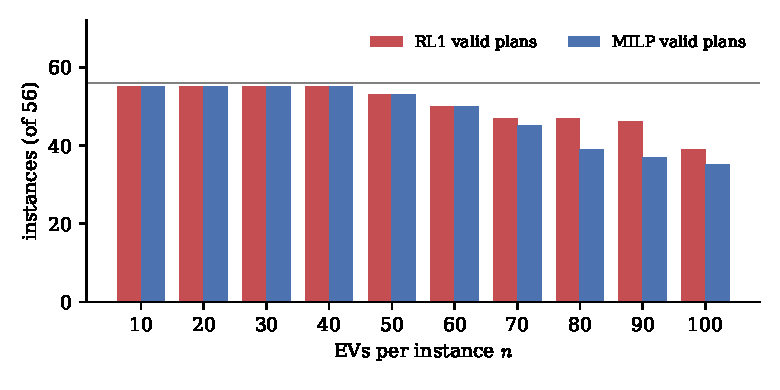
\includegraphics[width=0.7\textwidth]{figures/r_outcome.pdf}
\caption{Valid plans per instance size, RL1 against the MILP.}
\label{fig:outcome}
\end{figure}
\begin{table}[H]
\centering\small
\caption{Outcome per instance size and mean time per instance.}
\label{tab:outcome}
\begin{tabular}{@{}rrrrrrrr@{}}
\toprule
$n$ & instances & \shortstack[r]{RL1\\valid} & \shortstack[r]{RL1\\invalid} & \shortstack[r]{MILP\\valid} & \shortstack[r]{greedy\\valid} & \shortstack[r]{RL1 time\\(s)} & \shortstack[r]{MILP time\\(s)} \\
\midrule
10 & 56 & 55 & 1 & 55 & 55 & 0.03 & 0.1 \\
20 & 56 & 55 & 1 & 55 & 55 & 0.04 & 22.8 \\
30 & 56 & 55 & 1 & 55 & 55 & 0.06 & 96.5 \\
40 & 56 & 55 & 1 & 55 & 54 & 0.08 & 153.6 \\
50 & 56 & 53 & 3 & 53 & 52 & 0.11 & 181.9 \\
60 & 56 & 50 & 6 & 50 & 49 & 0.13 & 185.9 \\
70 & 56 & 47 & 9 & 45 & 44 & 0.15 & 191.1 \\
80 & 56 & 47 & 9 & 39 & 39 & 0.17 & 218.1 \\
90 & 56 & 46 & 10 & 37 & 37 & 0.19 & 235.5 \\
100 & 56 & 39 & 17 & 35 & 34 & 0.22 & 221.2 \\
\midrule
all & 560 & 502 & 58 & 479 & 474 & 0.12 & 150.7 \\
\bottomrule
\end{tabular}

\end{table}
\begin{table}[H]
\centering\small
\caption{RL1 outcome against the MILP outcome.}
\label{tab:crosstab}
\begin{tabular}{@{}lrrr@{}}
\toprule
MILP outcome & RL1 valid plan & RL1 invalid plan & instances \\
\midrule
optimal & 256 & 0 & 256 \\
time limit, plan & 223 & 0 & 223 \\
time limit, no plan & 23 & 7 & 30 \\
infeasible & 0 & 51 & 51 \\
\bottomrule
\end{tabular}

\end{table}
\begin{itemize}
  \item RL1 has a valid plan wherever the MILP has one, plus in \RLonly{} of the 30 instances the MILP left without a plan.
  \item Its \NInvalidR{} invalid plans are the \RLinvInf{} instances the data prove infeasible and \RLinvNoPlan{} of the MILP's unsolved instances.
\end{itemize}

\inshort{\NValidR{} valid RL1 plans against \NValidM{} for the MILP; every instance with a MILP plan also has an RL1 plan.}

\subsection{Instance-level overview}
\begin{table}[H]
\centering\footnotesize
\caption{Distribution of instance-level results over the valid RL1 plans (last column: MILP mean over its valid plans).}
\label{tab:inststats}
\begin{tabular}{@{}lrrrrrrrr@{}}
\toprule
measure (per instance) & count & mean & median & 10th pct & 90th pct & min & max & \shortstack[r]{MILP\\mean} \\
\midrule
objective $Z$ per EV (Rs) & 502 & 955 & 933 & 859 & 1092 & 818 & 1257 & 938 \\
operator share of $Z$ (\%) & 502 & 29.1 & 28.2 & 25.3 & 36.3 & 19.7 & 46.7 & 30.0 \\
vans used & 502 & 2.2 & 2.0 & 1.0 & 4.0 & 0.0 & 5.0 & 2.2 \\
EVs served by a van (\%) & 502 & 18.5 & 17.8 & 12.5 & 26.7 & 0.0 & 32.5 & 22.0 \\
free-choice EVs by van (\%) & 502 & 4.0 & 2.2 & 0.0 & 11.1 & 0.0 & 22.2 & 8.0 \\
mean FCS queue (min) & 502 & 2.22 & 0.04 & 0.00 & 8.78 & 0.00 & 17.25 & 0.99 \\
mean van wait (min) & 495 & 24.2 & 19.1 & 0.0 & 53.3 & 0.0 & 156.1 & 23.9 \\
mean request to charged (min) & 502 & 64.7 & 60.3 & 54.9 & 79.0 & 48.7 & 116.4 & 63.1 \\
van km & 502 & 72.7 & 69.5 & 22.9 & 126.0 & 0.0 & 246.0 & 71.2 \\
inference time (s) & 502 & 0.11 & 0.11 & 0.02 & 0.20 & 0.02 & 0.35 & -- \\
\bottomrule
\end{tabular}

\end{table}
\begin{figure}[H]
\centering
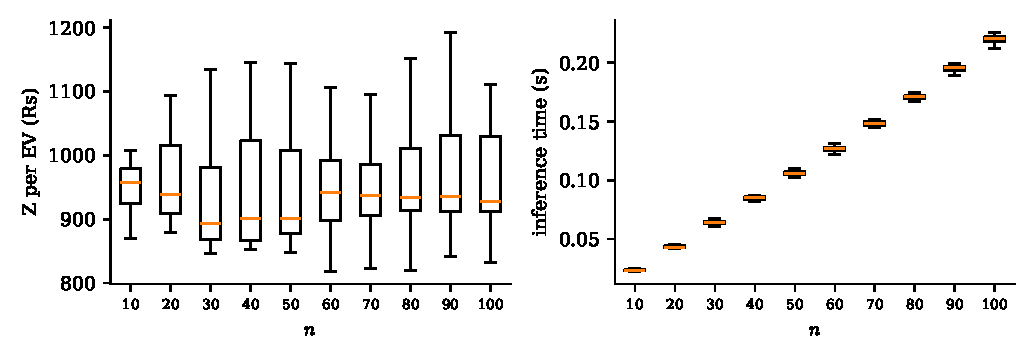
\includegraphics[width=0.85\textwidth]{figures/r_inst_by_n.pdf}
\caption{Objective per EV and inference time by instance size.}
\label{fig:instn}
\end{figure}
The objective per EV averages \ZperMeanR{} Rs (MILP \ZperMeanM{} Rs; the RL1 set also contains the 23 congested instances only RL1 solved). Inference stays below a second at every size (at most \RLtimeMax\,s).

\subsection{Families}
\begin{table}[H]
\centering\footnotesize
\caption{RL1 results by Solomon family.}
\label{tab:family}
\begin{tabular}{@{}lrrrrrrrrrr@{}}
\toprule
family & inst. & \shortstack[r]{RL1\\valid} & \shortstack[r]{MILP\\valid} & \shortstack[r]{Z per EV\\(Rs)} & \shortstack[r]{operator\\share (\%)} & \shortstack[r]{free-choice\\by van (\%)} & \shortstack[r]{mean queue\\(min)} & \shortstack[r]{request to\\charged (min)} & \shortstack[r]{vans\\used} & \shortstack[r]{gap to\\MILP (\%)} \\
\midrule
C1 & 90 & 90 & 90 & 930 & 29.2 & 2.2 & 1.46 & 64.7 & 2.16 & 1.06 \\
C2 & 80 & 80 & 79 & 948 & 28.3 & 6.1 & 1.73 & 65.7 & 1.88 & 1.60 \\
R1 & 120 & 89 & 76 & 941 & 30.7 & 2.5 & 5.99 & 66.2 & 2.63 & 0.80 \\
R2 & 110 & 110 & 110 & 881 & 29.1 & 2.4 & 2.69 & 64.5 & 1.99 & 1.22 \\
RC1 & 80 & 53 & 44 & 1092 & 27.0 & 5.3 & 6.72 & 82.7 & 2.62 & 1.13 \\
RC2 & 80 & 80 & 80 & 1015 & 29.3 & 4.3 & 1.75 & 67.6 & 2.21 & 0.60 \\
\bottomrule
\end{tabular}

\end{table}
RL1 gains most feasibility in the short-horizon families R1 and RC1, where the MILP runs out of time. The gap to the MILP is smallest in RC2 and R1 and largest in C2.

\subsection{EV-level distributions}
\begin{table}[H]
\centering\footnotesize
\caption{EV-level variables in valid RL1 plans (last column: MILP mean).}
\label{tab:evstats}
\begin{tabular}{@{}lrrrrrrr@{}}
\toprule
variable (per EV) & count & mean & median & 10th pct & 90th pct & max & \shortstack[r]{MILP\\mean} \\
\midrule
income $\theta$ & 26240 & 0.50 & 0.51 & 0.18 & 0.81 & 0.98 & 0.50 \\
drive to FCS (km), FCS users & 21509 & 2.46 & 1.77 & 0.72 & 5.07 & 23.77 & 2.28 \\
FCS queue (min), FCS users & 21509 & 3.04 & 0.00 & 0.00 & 9.21 & 56.82 & 1.37 \\
van wait (min), van users & 4731 & 29.1 & 0.0 & 0.0 & 92.9 & 412.4 & 26.5 \\
charging time (min) & 26240 & 51.0 & 44.0 & 31.0 & 75.7 & 109.1 & 50.7 \\
request to charged (min) & 26240 & 66.4 & 61.3 & 41.4 & 99.5 & 455.6 & 64.2 \\
money paid (Rs) & 26240 & 336 & 326 & 232 & 510 & 1000 & 341 \\
perceived money (Rs) & 26240 & 335 & 316 & 192 & 501 & 1000 & 338 \\
perceived time (Rs) & 26240 & 357 & 326 & 121 & 620 & 1881 & 328 \\
perceived total (Rs) & 26240 & 692 & 646 & 439 & 1017 & 2287 & 666 \\
\bottomrule
\end{tabular}

\end{table}
\begin{figure}[H]
\centering
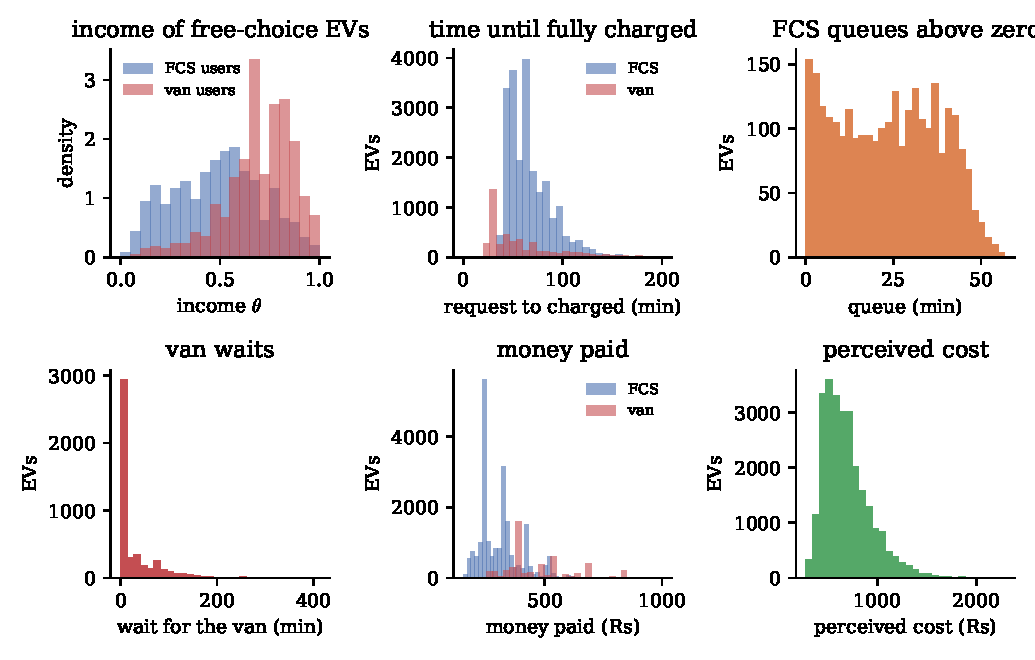
\includegraphics[width=\textwidth]{figures/r_ev_dists.pdf}
\caption{Distributions of income, time until charged, queues, van waits, money paid and perceived cost in RL1 plans.}
\label{fig:evdists}
\end{figure}
Van users are richer than station users, as in the MILP, but the separation is weaker. \NQueuedR{} of \NFCSfreeR{} free-choice station users queue (MILP: \NQueuedM{} of 19147), and queues are longer.

\subsection{Correlations}
\begin{figure}[H]
\centering
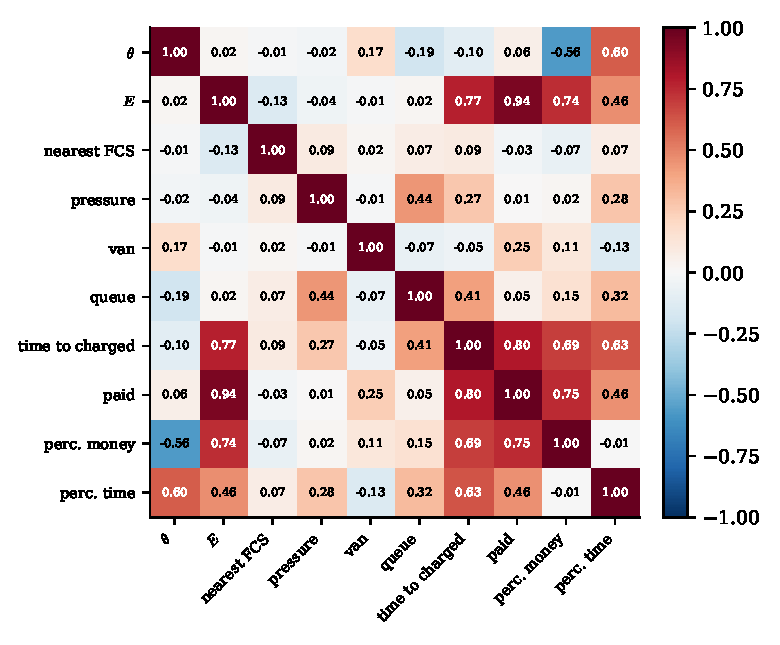
\includegraphics[width=0.62\textwidth]{figures/r_corr.pdf}
\caption{Spearman correlations between EV-level variables in RL1 plans (free-choice EVs).}
\label{fig:corr}
\end{figure}
The pattern is the MILP's (largest difference between the two matrices \CorrMaxDiff): income goes with vans ($\rho=\CorrThetaVanR$; MILP \CorrThetaVanM) and against queueing ($\rho=\CorrThetaQueueR$); demand pressure goes with queueing ($\rho=\CorrPressQueueR$). The weaker income--van link is the first sign of RL1's main difference.

\inshort{RL1 plans look like MILP plans in structure: the same correlations, the same kind of distributions, with weaker income--van separation and longer queues.}

%=====================================================================
\clearpage
\part{Comprehensive analysis}
\section{Analysis point by point}

%---------------------------------------------------------------------
\subsection{Training dynamics}
\label{sec:training}
\begin{figure}[H]
\centering
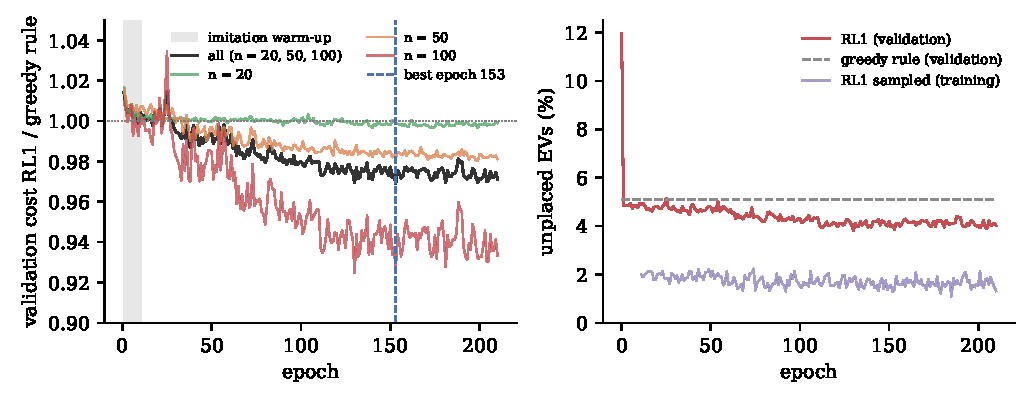
\includegraphics[width=\textwidth]{figures/r_training.pdf}
\caption{Left: validation cost of RL1 relative to the greedy rule, overall and by $n$; grey = imitation warm-up. Right: share of unplaced EVs.}
\label{fig:training}
\end{figure}
\begin{itemize}
  \item The untrained network costs \StartVal{} times the greedy rule. After \ImitEpochs{} epochs of imitation it is at \AfterImit: it copies the rule almost exactly.
  \item REINFORCE then improves on the rule. The best model (epoch \BestEpoch, after \Iters{} batches and \TrainBestS{} minutes) is \BestValPct\pct{} cheaper than the greedy rule on the validation instances (ratio \BestVal).
  \item The gain grows with size: ratio \ValTwenty{} at $n=20$, \ValFifty{} at $n=50$ and \ValHundred{} at $n=100$. Small instances leave little to improve; large ones offer more room.
  \item Unplaced EVs fall from about 5\pct{} (the greedy rule's level) to about 4\pct{} on the validation instances.
  \item Training stopped at epoch \Epochs{} (\TrainMin{} minutes on the \Device{} GPU): \StopReason.
\end{itemize}

\inshort{Imitation brings the network to the greedy rule in \ImitEpochs{} epochs; REINFORCE then makes it \BestValPct\pct{} cheaper than the rule, most of it at large $n$. Training took \TrainMin{} minutes and stopped early.}

%---------------------------------------------------------------------
\subsection{Solution quality against the MILP and the greedy rule}
\label{sec:quality}
\begin{figure}[H]
\centering
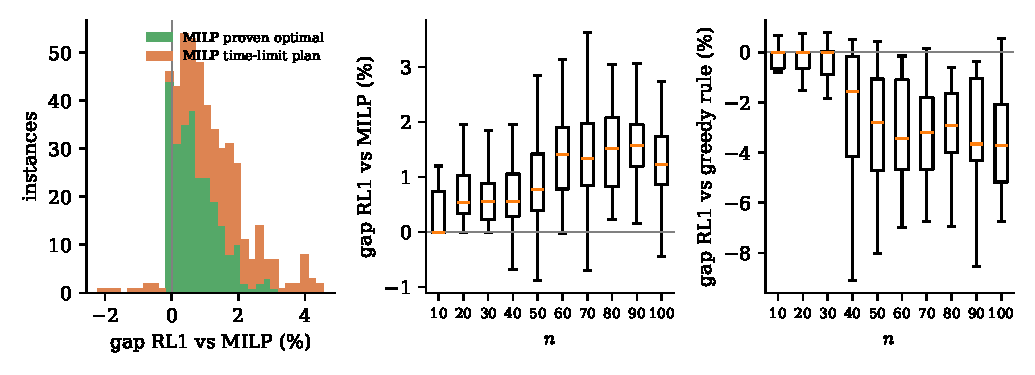
\includegraphics[width=\textwidth]{figures/r_gap.pdf}
\caption{Left: gap of RL1 to the MILP plan. Middle: by instance size. Right: gap of RL1 to the greedy rule.}
\label{fig:gap}
\end{figure}
\begin{table}[H]
\centering\footnotesize
\caption{Quality by instance size.}
\label{tab:qualityn}
\begin{tabular}{@{}lrrrrrrrrr@{}}
\toprule
group & inst. & \shortstack[r]{RL1\\valid} & \shortstack[r]{MILP\\valid} & \shortstack[r]{RL1 only\\valid} & \shortstack[r]{gap to MILP\\mean (\%)} & \shortstack[r]{gap to MILP\\median (\%)} & \shortstack[r]{gap to MILP\\max (\%)} & \shortstack[r]{gap to\\optimum (\%)} & \shortstack[r]{gap to\\greedy (\%)} \\
\midrule
$n=10$ & 56 & 55 & 55 & 0 & 0.50 & 0.00 & 2.79 & 0.50 & -1.60 \\
$n=20$ & 56 & 55 & 55 & 0 & 0.77 & 0.54 & 3.10 & 0.75 & -1.36 \\
$n=30$ & 56 & 55 & 55 & 0 & 0.69 & 0.55 & 2.59 & 0.53 & -1.03 \\
$n=40$ & 56 & 55 & 55 & 0 & 0.68 & 0.55 & 2.59 & 0.61 & -2.45 \\
$n=50$ & 56 & 53 & 53 & 0 & 0.97 & 0.77 & 3.83 & 0.64 & -3.14 \\
$n=60$ & 56 & 50 & 50 & 0 & 1.52 & 1.40 & 4.10 & 1.22 & -3.17 \\
$n=70$ & 56 & 47 & 45 & 2 & 1.60 & 1.34 & 4.55 & 1.19 & -3.13 \\
$n=80$ & 56 & 47 & 39 & 8 & 1.69 & 1.51 & 4.38 & 1.19 & -3.13 \\
$n=90$ & 56 & 46 & 37 & 9 & 1.59 & 1.58 & 4.18 & 1.41 & -3.35 \\
$n=100$ & 56 & 39 & 35 & 4 & 1.30 & 1.22 & 3.14 & 0.98 & -3.50 \\
\midrule
all & 560 & 502 & 479 & 23 & 1.07 & 0.89 & 4.55 & 0.74 & -2.47 \\
\bottomrule
\end{tabular}

\end{table}
\begin{table}[H]
\centering\footnotesize
\caption{Quality by family.}
\label{tab:qualityclass}
\begin{tabular}{@{}lrrrrrrrrr@{}}
\toprule
group & inst. & \shortstack[r]{RL1\\valid} & \shortstack[r]{MILP\\valid} & \shortstack[r]{RL1 only\\valid} & \shortstack[r]{gap to MILP\\mean (\%)} & \shortstack[r]{gap to MILP\\median (\%)} & \shortstack[r]{gap to MILP\\max (\%)} & \shortstack[r]{gap to\\optimum (\%)} & \shortstack[r]{gap to\\greedy (\%)} \\
\midrule
C1 & 90 & 90 & 90 & 0 & 1.06 & 1.01 & 4.00 & 0.74 & -1.12 \\
C2 & 80 & 80 & 79 & 1 & 1.60 & 1.58 & 4.10 & 1.44 & -1.04 \\
R1 & 120 & 89 & 76 & 13 & 0.80 & 0.45 & 3.94 & 0.34 & -1.96 \\
R2 & 110 & 110 & 110 & 0 & 1.22 & 0.99 & 4.38 & 0.66 & -2.57 \\
RC1 & 80 & 53 & 44 & 9 & 1.13 & 0.93 & 3.98 & 0.75 & -5.94 \\
RC2 & 80 & 80 & 80 & 0 & 0.60 & 0.41 & 4.55 & 0.19 & -4.01 \\
\midrule
all & 560 & 502 & 479 & 23 & 1.07 & 0.89 & 4.55 & 0.74 & -2.47 \\
\bottomrule
\end{tabular}

\end{table}
\begin{itemize}
  \item Over the \NBoth{} instances where both have a valid plan, RL1 is \GapMean\pct{} above the MILP on average (median \GapMed, range \GapMin{} to \GapMax\pct). \RLwithinOne\pct{} of RL1 plans are within 1\pct{} of the MILP and \RLwithinTwo\pct{} within 2\pct.
  \item Against the \NGapOpt{} proven optima the gap is \GapOptMean\pct; RL1 finds the optimum itself in \OptEqual{} instances, mostly at $n=10$.
  \item Against the \NGapTL{} MILP time-limit plans the gap is \GapTLMean\pct, and in \RLbetter{} of them RL1 is cheaper than the MILP, e.g.\ \BetterList.
  \item The gap grows from about 0.5--0.8\pct{} at $n\le40$ to about 1.3--1.7\pct{} at $n\ge60$.
  \item Against the greedy rule RL1 is cheaper in \GreedyBeat{} of \GreedyN{} instances, \GreedyGapAbs\pct{} cheaper on average. At $n\le30$ RL1 and the rule are often equal; from $n=40$ RL1 saves 2--4\pct.
\end{itemize}

\inshort{RL1 is about 1\pct{} above the MILP and 0.7\pct{} above proven optima, beats the MILP's unfinished plans in \RLbetter{} instances, and clearly beats the greedy rule from $n=40$ on.}

%---------------------------------------------------------------------
\subsection{Feasibility: where RL1 finds plans and where it fails}
\label{sec:feasibility}
\begin{table}[H]
\centering\small
\caption{The \RLonly{} instances where RL1 has a valid plan and the MILP none.}
\label{tab:rlonly}
\begin{tabular}{@{}lrlrrr@{}}
\toprule
file & $n$ & family & \shortstack[r]{$Z$ per EV\\(Rs)} & \shortstack[r]{mean queue\\(min)} & \shortstack[r]{vans\\used} \\
\midrule
RC106 & 70 & RC1 & 1058 & 6.89 & 4 \\
RC108 & 70 & RC1 & 1134 & 11.34 & 4 \\
R106 & 80 & R1 & 933 & 4.71 & 4 \\
R107 & 80 & R1 & 932 & 5.77 & 4 \\
R108 & 80 & R1 & 1050 & 13.11 & 5 \\
R109 & 80 & R1 & 979 & 8.18 & 4 \\
RC104 & 80 & RC1 & 1197 & 13.66 & 5 \\
RC106 & 80 & RC1 & 1098 & 7.03 & 5 \\
RC107 & 80 & RC1 & 1152 & 10.88 & 5 \\
RC108 & 80 & RC1 & 1185 & 11.37 & 5 \\
R106 & 90 & R1 & 965 & 7.76 & 4 \\
R107 & 90 & R1 & 1001 & 10.87 & 4 \\
R108 & 90 & R1 & 1121 & 16.90 & 5 \\
R109 & 90 & R1 & 1016 & 10.77 & 5 \\
R111 & 90 & R1 & 1033 & 12.25 & 5 \\
R112 & 90 & R1 & 1117 & 17.25 & 5 \\
RC104 & 90 & RC1 & 1228 & 16.51 & 5 \\
RC107 & 90 & RC1 & 1192 & 10.63 & 5 \\
RC108 & 90 & RC1 & 1254 & 15.13 & 5 \\
C204 & 100 & C2 & 1257 & 11.42 & 5 \\
R109 & 100 & R1 & 1039 & 12.02 & 5 \\
R110 & 100 & R1 & 1110 & 15.78 & 5 \\
R111 & 100 & R1 & 1062 & 14.92 & 5 \\
\bottomrule
\end{tabular}

\end{table}
\begin{table}[H]
\centering\small
\caption{Invalid RL1 plans.}
\label{tab:invalid}
\begin{tabular}{@{}lrrrrr@{}}
\toprule
family & RL1 invalid & MILP: infeasible & MILP: no plan & \shortstack[r]{broken limits\\per plan} & smallest $n$ \\
\midrule
R1 & 31 & 29 & 2 & 3.0 & 50 \\
RC1 & 27 & 22 & 5 & 4.3 & 10 \\
\bottomrule
\end{tabular}

\end{table}
\begin{table}[H]
\centering\small
\caption{Limits broken in invalid RL1 plans.}
\label{tab:violations}
\begin{tabular}{@{}lr@{}}
\toprule
broken limit (first three listed per plan) & count \\
\midrule
EV finishes after T & 63 \\
van back after T & 43 \\
queue above W & 11 \\
\bottomrule
\end{tabular}

\end{table}
\begin{itemize}
  \item The \RLonly{} instances only RL1 solved are the most congested ones: R1 and RC1 at $n=70$--100 and C204 at $n=100$, with 4--5 vans and mean queues of 5--17 minutes. The MILP's greedy warm start fails there and Gurobi finds no plan in 300\,s; RL1's learned policy does.
  \item All \InvR{} invalid plans are on instances without any MILP plan: the \RLinvInf{} data-infeasible ones (no plan can exist) and \RLinvNoPlan{} unsolved ones. They break \InvViolMean{} limits on average, mostly an EV finishing after $T$ or a van returning after $T$.
\end{itemize}

\inshort{RL1 is the more reliable plan finder: it never fails where the MILP succeeds and succeeds on \RLonly{} of the MILP's 30 unsolved instances.}

%---------------------------------------------------------------------
\subsection{Computation and the value of learning}
\label{sec:compute}
\begin{figure}[H]
\centering
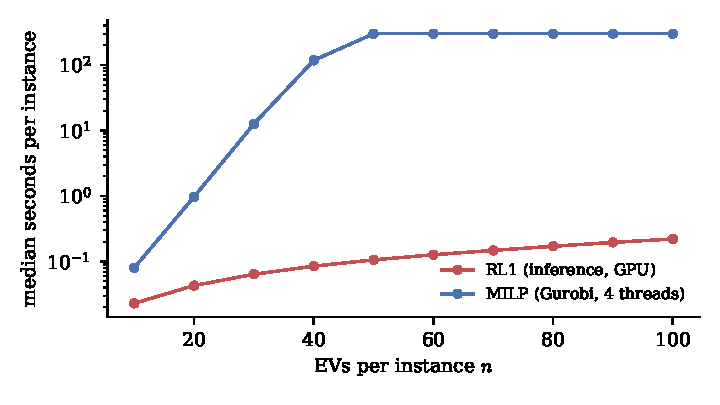
\includegraphics[width=0.66\textwidth]{figures/r_time.pdf}
\caption{Median time per instance (log scale).}
\label{fig:time}
\end{figure}
RL1 solves an instance in \RLtime\,s on average against \MILPtime\,s for the MILP, about \Speedup{} times faster; all 560 instances take \RLtotalS\,s against \MILPtotalH{} hours. The cost is moved to training: \TrainS\,s to the best model, which equals the MILP time of about \BreakEven{} instances. After that, every new instance is almost free, and the trained network also handles sizes and layouts it has not seen.

\inshort{Learning trades a one-off training cost (about half an hour) for near-instant solving; it pays off after about \BreakEven{} instances.}

%---------------------------------------------------------------------
\subsection{Anatomy of the objective: where RL1 loses}
\label{sec:anatomy}
\begin{table}[H]
\centering\small
\caption{Terms of $Z$ over the \NBoth{} instances where both have a valid plan.}
\label{tab:terms}
\begin{tabular}{@{}lrrrrr@{}}
\toprule
term & \shortstack[r]{MILP\\Rs per plan} & \shortstack[r]{RL1\\Rs per plan} & \shortstack[r]{RL1 $-$ MILP\\(\% of $Z$)} & \shortstack[r]{MILP\\share (\%)} & \shortstack[r]{RL1\\share (\%)} \\
\midrule
$Z_1$ EV driving & 386 & 393 & +0.02 & 0.8 & 0.8 \\
$Z_2$ van driving & 1067 & 1063 & -0.01 & 2.3 & 2.2 \\
$Z_3$ van dispatch & 3254 & 3147 & -0.23 & 6.9 & 6.6 \\
$Z_4$ operator energy & 9283 & 9193 & -0.19 & 19.6 & 19.2 \\
$Z_5$ tariff & 16723 & 16528 & -0.41 & 35.3 & 34.5 \\
$Z_6$ time & 16596 & 17598 & +2.12 & 35.1 & 36.7 \\
\midrule
$Z$ & 47308 & 47922 & +1.30 & 100.0 & 100.0 \\
\bottomrule
\end{tabular}

\end{table}
\begin{figure}[H]
\centering
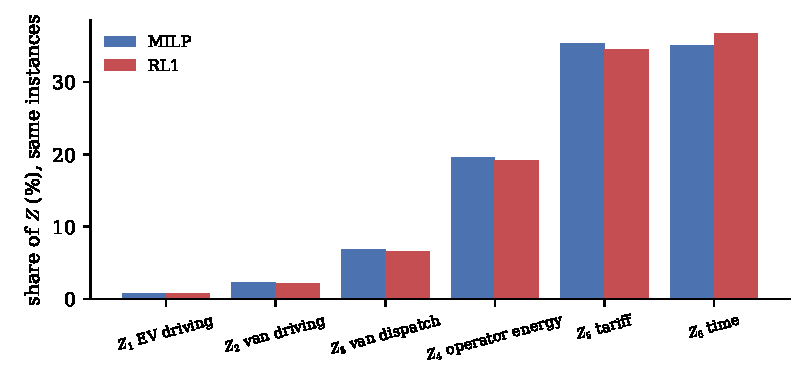
\includegraphics[width=0.7\textwidth]{figures/r_obj_compare.pdf}
\caption{Composition of $Z$, MILP against RL1 (same instances).}
\label{fig:obj}
\end{figure}
Summed over the common instances RL1's $Z$ is \ExtraTotal\pct{} higher. The perceived time term carries all of it and more (\ExtraTime\pct{} of $Z$), while RL1 saves on the perceived tariff (\ExtraTariff), operator energy (\ExtraEnergy), van dispatch (\ExtraDispatch), van driving (\ExtraVanKm) and pays slightly more for EV driving (\ExtraDrive). Fewer free-choice customers on vans means cheaper energy and tariffs but longer queues and charging at the stations.

\subsubsection{Elasticities (envelope theorem)}
\begin{table}[H]
\centering\small
\caption{Elasticity of $Z$ with respect to every coefficient, MILP and RL1 (same instances).}
\label{tab:elasticity}
\begin{tabular}{@{}lrrrr@{}}
\toprule
coefficient & value & MILP elasticity (\%) & RL1 elasticity (\%) & difference \\
\midrule
$\mu^{0}$ & 1.5 & 26.87 & 26.35 & -0.52 \\
$p^{\mathrm F}$ & 15 & 25.67 & 25.95 & +0.28 \\
$c^{\mathrm{C},1}$ & 10 & 22.01 & 23.01 & +1.00 \\
$\pi^{\mathrm F}$ & 8.7 & 14.61 & 14.93 & +0.32 \\
$p^{\mathrm M}$ & 25 & 9.68 & 8.54 & -1.14 \\
$\mu^{1}$ & 0.5 & 9.29 & 8.96 & -0.34 \\
$c^{\mathrm F}_m$ & 1500 & 6.88 & 6.57 & -0.31 \\
$\pi^{\mathrm M}$ & 10.7 & 5.02 & 4.26 & -0.76 \\
$c^{\mathrm{D},1}$ & 15 & 4.91 & 5.35 & +0.44 \\
$c^{\mathrm{V},1}$ & 5 & 3.75 & 3.13 & -0.62 \\
$c^{\mathrm{C},0}$ & 1 & 2.38 & 2.38 & +0.00 \\
$c^{\mathrm M}$ & 15 & 2.26 & 2.22 & -0.04 \\
$c^{\mathrm{Q},1}$ & 25 & 0.86 & 1.59 & +0.73 \\
$c^{\mathrm{EV}}$ & 4 & 0.81 & 0.82 & +0.00 \\
$c^{\mathrm{D},0}$ & 1.5 & 0.62 & 0.61 & -0.01 \\
$c^{\mathrm{V},0}$ & 0.5 & 0.34 & 0.31 & -0.04 \\
$c^{\mathrm{Q},0}$ & 2.5 & 0.20 & 0.35 & +0.14 \\
\bottomrule
\end{tabular}

\end{table}
\begin{figure}[H]
\centering
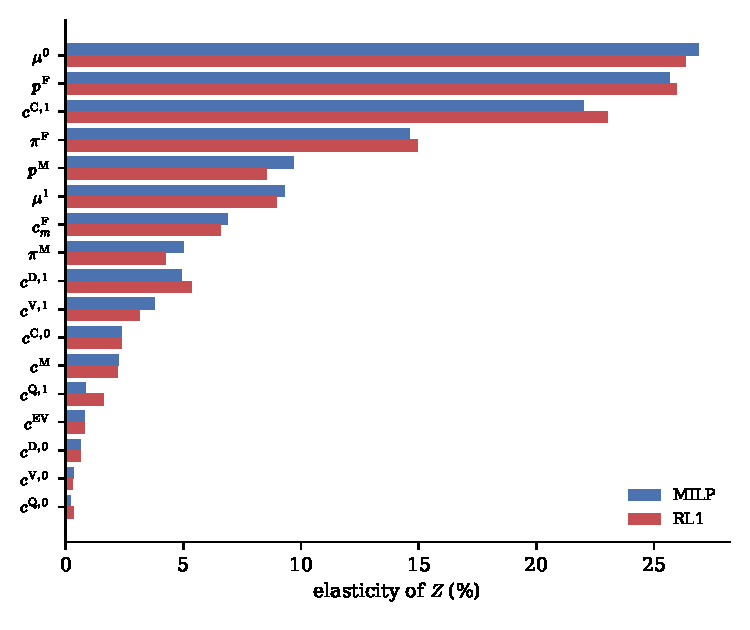
\includegraphics[width=0.6\textwidth]{figures/r_elasticity.pdf}
\caption{Elasticities of $Z$, MILP against RL1.}
\label{fig:elasticity}
\end{figure}
The elasticities are almost identical (largest difference \ElDiffMax{} points, for \ElDiffMaxName: RL1 \ElPMR, MILP \ElPMM). The most influential coefficients are again $p^{\mathrm F}$ (\ElPFR\pct), $\mu^{0}$ (\ElMuZeroR\pct), $c^{\mathrm{C},1}$ (\ElCCOneR\pct) and $\pi^{\mathrm F}$ (\ElPiFR\pct). The cost structure of RL1 plans is the MILP's; what differs is a small shift from van to station.

\inshort{RL1 loses on waiting time and gains a little on tariff, energy and dispatch; its sensitivity to every coefficient is the MILP's.}

%---------------------------------------------------------------------
\subsection{Decision agreement with the MILP}
\label{sec:agreement}
\begin{table}[H]
\centering\small
\caption{Resource type chosen for free-choice EVs, MILP against RL1 (same instances).}
\label{tab:confusion}
\begin{tabular}{@{}lrrr@{}}
\toprule
MILP resource $\downarrow$ / RL1 resource $\rightarrow$ & FCS & van & agreement (\%) \\
\midrule
FCS & 18752 & 395 & 97.9 \\
van & 1134 & 303 & 21.1 \\
\bottomrule
\end{tabular}

\end{table}
\begin{figure}[H]
\centering
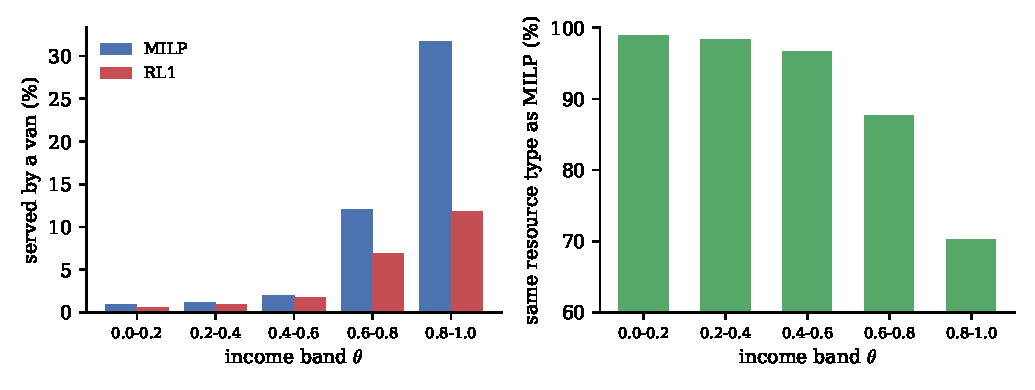
\includegraphics[width=\textwidth]{figures/r_agreement.pdf}
\caption{Left: van share by income band. Right: share of free-choice EVs with the same resource type as in the MILP plan.}
\label{fig:agreement}
\end{figure}
\begin{itemize}
  \item RL1 chooses the same resource type as the MILP for \AgreeType\pct{} of free-choice EVs (\AgreeTypeOpt\pct{} on proven-optimal instances); where both use a station, it is the same station in \AgreeStation\pct.
  \item The disagreement is one-sided. When the MILP sends a free-choice EV to a station, RL1 does too in \AgreeFcsFcs\pct; when the MILP gives it a van, RL1 does only in \AgreeVanVan\pct{} (\RLfcsMILPvan{} EVs that the MILP put on a van RL1 sent to a station; only \RLvanMILPfcs{} the other way).
  \item Agreement falls with income from \AgreeBandMax\pct{} to \AgreeBandMin\pct: exactly the high-income customers whom the MILP puts on vans.
\end{itemize}

\inshort{RL1 agrees with the MILP on most decisions; it misses the MILP's vans for rich free-choice customers.}

%---------------------------------------------------------------------
\subsection{Income and the choice of resource}
\label{sec:income}
\begin{figure}[H]
\centering
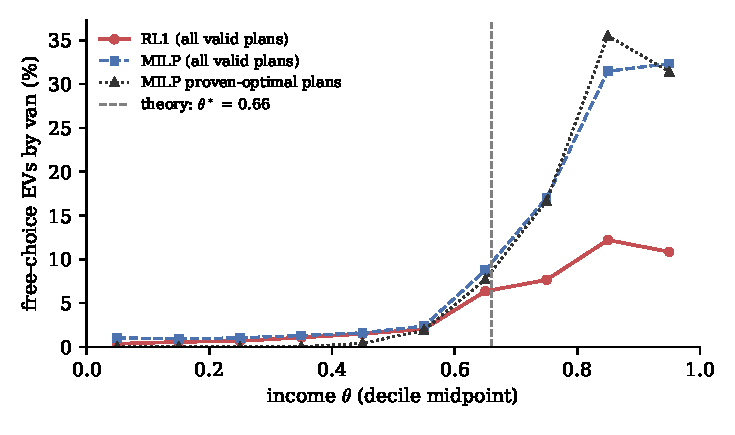
\includegraphics[width=0.7\textwidth]{figures/r_van_by_income.pdf}
\caption{Share of free-choice EVs served by a van by income decile: RL1, MILP, MILP proven optima, and the theoretical threshold.}
\label{fig:van}
\end{figure}
\begin{table}[H]
\centering\small
\caption{Van share by income decile.}
\label{tab:deciles}
\begin{tabular}{@{}lrrrrr@{}}
\toprule
income $\theta$ & \shortstack[r]{EVs\\(RL1)} & \shortstack[r]{RL1 by\\van (\%)} & \shortstack[r]{RL1 95\,\%\\interval} & \shortstack[r]{MILP by\\van (\%)} & \shortstack[r]{MILP optimal\\by van (\%)} \\
\midrule
0.0--0.1 & 564 & 0.4 & [0.1, 1.3] & 1.0 & 0.0 \\
0.1--0.2 & 2326 & 0.6 & [0.3, 1.0] & 0.9 & 0.0 \\
0.2--0.3 & 2230 & 0.7 & [0.4, 1.1] & 1.0 & 0.0 \\
0.3--0.4 & 2442 & 1.1 & [0.7, 1.6] & 1.3 & 0.0 \\
0.4--0.5 & 3358 & 1.5 & [1.1, 2.0] & 1.6 & 0.4 \\
0.5--0.6 & 4002 & 2.0 & [1.6, 2.5] & 2.4 & 1.9 \\
0.6--0.7 & 3155 & 6.3 & [5.5, 7.2] & 8.7 & 7.7 \\
0.7--0.8 & 2079 & 7.6 & [6.6, 8.9] & 17.0 & 16.6 \\
0.8--0.9 & 1517 & 12.2 & [10.6, 13.9] & 31.5 & 35.5 \\
0.9--1.0 & 636 & 10.8 & [8.7, 13.5] & 32.3 & 31.4 \\
\bottomrule
\end{tabular}

\end{table}
\begin{table}[H]
\centering\small
\caption{Logistic regression of $P(\text{served by a van})$ in RL1 plans (last column: MILP).}
\label{tab:logit}
\begin{tabular}{@{}lrrrrr@{}}
\toprule
term & RL1 coef. & std.\ error & $z$ & $p$-value & MILP coef. \\
\midrule
intercept & -8.043 & 0.291 & -27.6 & $<0.001$ & -9.036 \\
income $\theta$ & 7.504 & 0.326 & 23.0 & $<0.001$ & 9.806 \\
medium pressure & -1.268 & 0.125 & -10.1 & $<0.001$ & -0.851 \\
high pressure & 3.394 & 0.301 & 11.3 & $<0.001$ & 3.839 \\
$\theta\times$ high pressure & -5.040 & 0.424 & -11.9 & $<0.001$ & -5.715 \\
long horizon (type 2) & 0.311 & 0.082 & 3.8 & $<0.001$ & -0.030 \\
energy $E_i$ (per 10 kWh) & -0.070 & 0.065 & -1.1 & 0.285 & -0.250 \\
nearest reachable FCS (km) & 0.079 & 0.047 & 1.7 & 0.091 & 0.449 \\
\bottomrule
\end{tabular}

\end{table}
\begin{itemize}
  \item RL1 learned the income threshold: the van share is near zero below $\theta=0.6$ and starts to rise at $\theta$ \StepR, where the formulation predicts $\theta^{*}=0.66$ (MILP report, Section 4.3).
  \item The step is smaller: \VanSixEightR\pct{} at $\theta$ 0.6--0.8 and \VanTopR\pct{} at 0.8--1.0, against \VanTopM\pct{} in the MILP. Overall \VanAllR\pct{} of free-choice EVs get a van (MILP \VanAllM\pct); van users have mean income \ThetaVanR, station users \ThetaFCSR.
  \item $+0.1$ in $\theta$ raises the probability of a van by \AMER{} percentage points on average (MILP \AMEM); \AMEnotR{} at low or medium pressure and \AMEhighR{} at high pressure. The regression classifies \AccR\pct{} of EVs correctly. Income, demand pressure and their interaction have the MILP's signs. Unlike in the MILP, the long horizon has an effect of its own (RL1 uses more vans in type-2 families beyond what congestion explains), and distance to the station and energy demand are not significant: RL1 bases its van choices less on the EV's own situation than the MILP does.
\end{itemize}

\inshort{RL1 found the same income threshold as theory and the MILP, but acts on it about half as strongly.}

%---------------------------------------------------------------------
\subsection{Shadow prices of RL1 plans}
\label{sec:duals}
The fixed-plan LP of the MILP report works for any plan: fix the decisions, re-solve the start times and waits, read the duals. For all \NValidR{} RL1 plans the LP value equals the plan's own waiting cost, so RL1's earliest-start timing is optimal for its decisions.
\begin{table}[H]
\centering\footnotesize
\caption{Shadow prices of the fixed-plan LPs, RL1 and MILP.}
\label{tab:duals}
\resizebox{\textwidth}{!}{\begin{tabular}{@{}lrrrrrrp{3.0cm}@{}}
\toprule
constraint & RL1 rows & \shortstack[r]{RL1 non-\\zero (\%)} & \shortstack[r]{RL1 mean\\(Rs/min)} & \shortstack[r]{RL1 max\\(Rs/min)} & \shortstack[r]{MILP non-\\zero (\%)} & \shortstack[r]{MILP mean\\(Rs/min)} & meaning \\
\midrule
gun order $S_j\ge S_i+\tau^{\mathrm F}_i$ & 12521 & 22.1 & 13.81 & 60.26 & 13.0 & 11.63 & value of one gun-minute \\
van order $S_j\ge S_i+\tau^{\mathrm M}_i+t_{ij}$ & 3618 & 43.2 & 4.58 & 18.78 & 40.6 & 4.50 & value of one van-minute \\
first stop $S_a\ge t_{0a}$ & 1113 & 69.1 & 6.63 & 20.91 & 73.1 & 7.36 & value of an earlier departure \\
FCS arrival $S_i\ge r_i+t_{if}$ & 21509 & 11.1 & 13.75 & 60.26 & 7.7 & 11.51 & not unique (degenerate) \\
van release $S_i\ge r_i$ & 4731 & 50.5 & 3.69 & 18.57 & 52.7 & 3.80 & not unique (degenerate) \\
queue limit $q^{\mathrm F}_i\le W_i$ & 21509 & 0.0 & 0.00 & 0.00 & 0.0 & 0.00 & value of patience \\
deadline $C_i\le T$, van return & 27353 & 0.0 & 0.00 & 0.00 & 0.0 & 0.00 & value of horizon \\
\bottomrule
\end{tabular}
}
\end{table}
\begin{figure}[H]
\centering
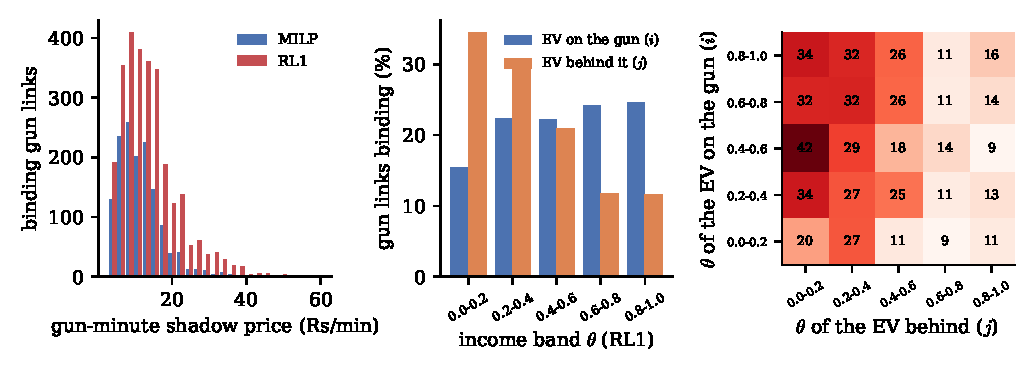
\includegraphics[width=\textwidth]{figures/r_gun_duals.pdf}
\caption{Left: gun-minute shadow prices where non-zero. Middle and right: binding gun links in RL1 plans by income of the EV on the gun and of the EV behind it.}
\label{fig:gunduals}
\end{figure}
\begin{table}[H]
\centering\small
\caption{Gun links in RL1 plans by demand pressure of the EV behind.}
\label{tab:gunpressure}
\begin{tabular}{@{}lrrrr@{}}
\toprule
\shortstack[l]{demand pressure\\of the follower} & gun links & \shortstack[r]{binding\\(\%)} & \shortstack[r]{mean dual if\\binding (Rs/min)} & \shortstack[r]{mean dual\\all links (Rs/min)} \\
\midrule
low & 5629 & 0.9 & 13.7 & 0.13 \\
medium & 3473 & 5.2 & 12.5 & 0.65 \\
high & 3419 & 74.2 & 13.9 & 10.31 \\
\bottomrule
\end{tabular}

\end{table}
\begin{figure}[H]
\centering
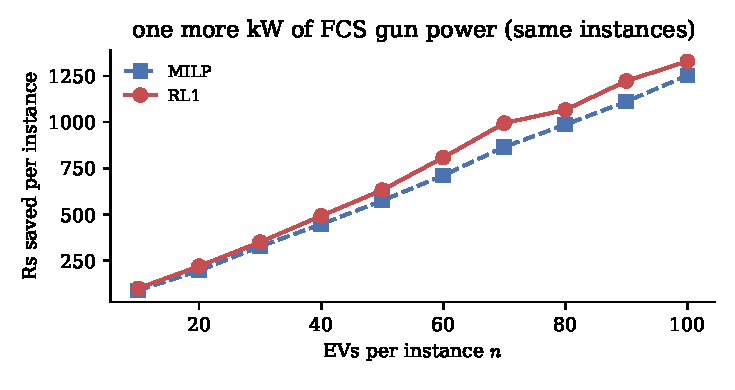
\includegraphics[width=0.66\textwidth]{figures/r_power.pdf}
\caption{Value of one more kW of station-gun power, RL1 against MILP plans of the same instances.}
\label{fig:power}
\end{figure}
\begin{itemize}
  \item \textbf{Gun-minutes are scarcer in RL1 plans:} \GunBindR\pct{} of gun links are binding (MILP \GunBindM\pct), worth \GunMeanR{} Rs/min on average when binding (MILP \GunMeanM). At high demand pressure \GunBindHighR\pct{} are binding, at low pressure \GunBindLowR\pct.
  \item \textbf{The same priority pattern:} a gun link is binding in \GunOccTopR\pct{} of cases when the EV on the gun is in the richest band and \GunOccBotR\pct{} in the poorest; seen from behind, \GunFolBotR\pct{} for the poorest and \GunFolTopR\pct{} for the richest.
  \item \textbf{Van-minutes:} \VanBindR\pct{} of van legs binding, \VanMeanR{} Rs/min when binding, close to the MILP.
  \item \textbf{Patience and deadline:} again zero shadow price in every plan (\PatNZR{} and \DeadNZR{} non-zero); they act only by ruling out decisions.
  \item \textbf{Value of power:} one more kW of station-gun power is worth \DPFpairR{} Rs per instance in RL1 plans against \DPFpairM{} Rs in the MILP plans of the same instances; \DPFcongR\pct{} of it is congestion relief (MILP report: 12.3\pct). A congested plan gains more from faster guns.
\end{itemize}

\inshort{RL1 plans have the same shadow-price structure as MILP plans, with more scarce gun-minutes: they queue more, so faster guns would help them more.}

%---------------------------------------------------------------------
\subsection{Queues, priority and driving}
\label{sec:queues}
\begin{figure}[H]
\centering
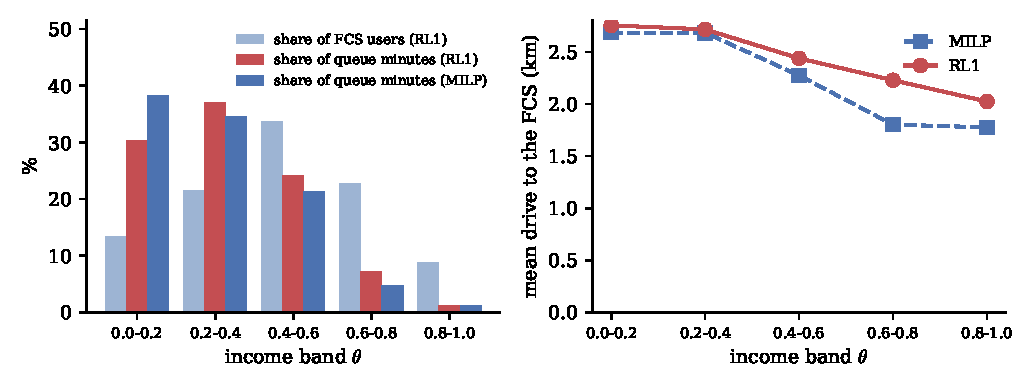
\includegraphics[width=\textwidth]{figures/r_queues.pdf}
\caption{Left: share of station users and of queue minutes by income band (RL1 and MILP). Right: mean distance to the station.}
\label{fig:queues}
\end{figure}
\begin{table}[H]
\centering\footnotesize
\caption{Station users by income band in RL1 plans (last columns: MILP).}
\label{tab:queues}
\begin{tabular}{@{}lrrrrrrrr@{}}
\toprule
income $\theta$ & \shortstack[r]{RL1 FCS\\users} & \shortstack[r]{share of\\users (\%)} & \shortstack[r]{share of queue\\minutes (\%)} & \shortstack[r]{queueing\\(\%)} & \shortstack[r]{mean queue\\(min)} & \shortstack[r]{drive to\\FCS (km)} & \shortstack[r]{MILP share of\\queue min. (\%)} & \shortstack[r]{MILP drive\\(km)} \\
\midrule
0.0--0.2 & 2875 & 13.4 & 30.2 & 21.4 & 6.88 & 2.76 & 38.2 & 2.69 \\
0.2--0.4 & 4631 & 21.5 & 37.1 & 19.1 & 5.24 & 2.72 & 34.6 & 2.69 \\
0.4--0.6 & 7229 & 33.6 & 24.2 & 11.3 & 2.19 & 2.44 & 21.3 & 2.27 \\
0.6--0.8 & 4875 & 22.7 & 7.2 & 6.8 & 0.96 & 2.23 & 4.7 & 1.80 \\
0.8--1.0 & 1899 & 8.8 & 1.3 & 6.4 & 0.44 & 2.02 & 1.1 & 1.78 \\
\bottomrule
\end{tabular}

\end{table}
The poorest 40\pct{} are \UShareBottomR\pct{} of station users and do \QShareBottomR\pct{} of the queueing (MILP \QShareBottomM\pct); the richest 20\pct{} do \QShareTopR\pct{} (MILP \QShareTopM\pct). RL1 keeps the MILP's priority order: the customer with the higher queueing rate goes first. Station users drive a little farther than in the MILP (\DriveBotR{} against \DriveBotM{} km in the poorest band, \DriveTopR{} against \DriveTopM{} km in the richest), as the richer customers the MILP would put on vans now compete for the near stations.

\inshort{The same queue priority as the MILP; more customers at the stations means longer queues and drives for everybody.}

%---------------------------------------------------------------------
\subsection{Peak and off-peak: demand pressure}
\label{sec:pressure}
\begin{figure}[H]
\centering
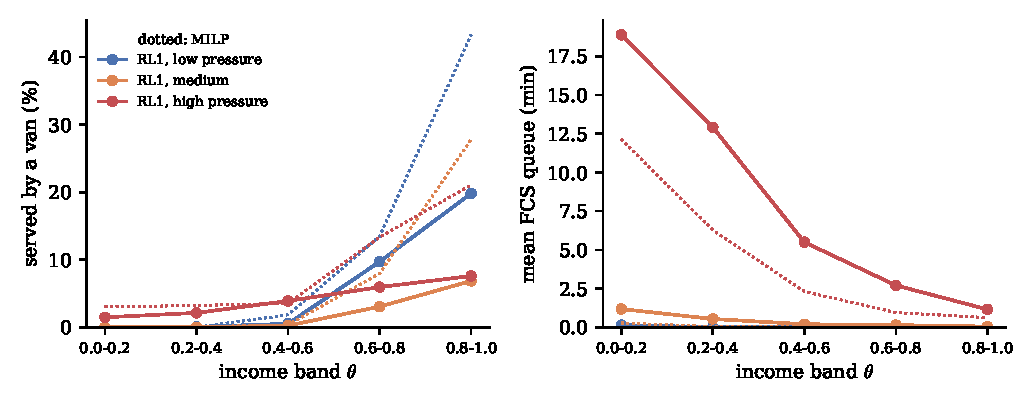
\includegraphics[width=\textwidth]{figures/r_pressure.pdf}
\caption{Van share and mean station queue by income band and demand pressure; solid RL1, dotted MILP.}
\label{fig:pressure}
\end{figure}
\begin{table}[H]
\centering\scriptsize
\caption{Free-choice EVs in RL1 plans by demand pressure (last columns: MILP).}
\label{tab:pressure}
\resizebox{\textwidth}{!}{\begin{tabular}{@{}lrrrrrrrrrrr@{}}
\toprule
\shortstack[l]{demand\\pressure} & EVs & \shortstack[r]{queueing\\(\%)} & \shortstack[r]{mean queue\\(min)} & \shortstack[r]{by van\\(\%)} & \shortstack[r]{by van\\$\theta$ 0.0--0.2} & \shortstack[r]{by van\\$\theta$ 0.2--0.4} & \shortstack[r]{by van\\$\theta$ 0.4--0.6} & \shortstack[r]{by van\\$\theta$ 0.6--0.8} & \shortstack[r]{by van\\$\theta$ 0.8--1.0} & \shortstack[r]{MILP mean\\queue (min)} & \shortstack[r]{MILP top\\band van (\%)} \\
\midrule
low & 8245 & 0.7 & 0.06 & 4.7 & 0.0 & 0.1 & 0.5 & 9.7 & 19.8 & 0.03 & 43.3 \\
medium & 5816 & 3.1 & 0.37 & 1.5 & 0.0 & 0.0 & 0.2 & 3.1 & 6.9 & 0.08 & 27.8 \\
high & 8248 & 32.0 & 7.94 & 4.0 & 1.5 & 2.1 & 3.9 & 6.0 & 7.6 & 4.08 & 21.1 \\
\bottomrule
\end{tabular}
}
\end{table}
\begin{itemize}
  \item Queues appear at high pressure as in the MILP but are about twice as long: \QRHigh{} min on average (MILP \QMHigh), \LowQRHigh{} min for the poorest 40\pct{} (MILP \LowQMHigh) and \TopQRHigh{} min for the richest band.
  \item The richest band's van share falls with pressure as in the MILP but from a lower level: \TopRLow\pct{} at low and \TopRHigh\pct{} at high pressure (MILP \TopMLow{} and \TopMHigh\pct).
\end{itemize}

\inshort{At peak RL1 still protects the rich in the queue, but with fewer vans the queues of everybody grow.}

%---------------------------------------------------------------------
\subsection{Planning horizon and layout}
\label{sec:horizon}
\begin{figure}[H]
\centering
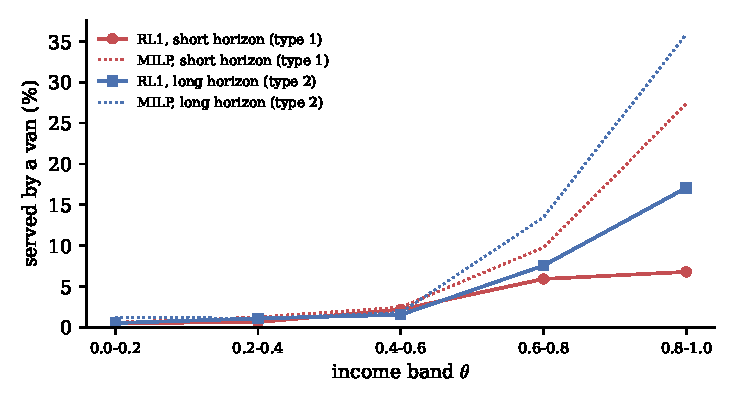
\includegraphics[width=0.7\textwidth]{figures/r_horizon.pdf}
\caption{Van share by income band, short against long horizon; solid RL1, dotted MILP.}
\label{fig:horizon}
\end{figure}
\begin{table}[H]
\centering\scriptsize
\caption{Van share by family and income band in RL1 plans (last column: MILP top band).}
\label{tab:families}
\begin{tabular}{@{}llrrrrrrrrr@{}}
\toprule
family & horizon & EVs & \shortstack[r]{mean\\pressure} & \shortstack[r]{by van\\(\%)} & \shortstack[r]{by van\\$\theta$ 0.0--0.2} & \shortstack[r]{by van\\$\theta$ 0.2--0.4} & \shortstack[r]{by van\\$\theta$ 0.4--0.6} & \shortstack[r]{by van\\$\theta$ 0.6--0.8} & \shortstack[r]{by van\\$\theta$ 0.8--1.0} & \shortstack[r]{MILP\\top band} \\
\midrule
C1 & short & 4104 & 0.38 & 2.2 & 0.7 & 0.9 & 1.0 & 2.9 & 6.9 & 37.0 \\
C2 & long & 3856 & 0.32 & 6.1 & 0.9 & 1.0 & 1.3 & 11.2 & 21.1 & 36.8 \\
R1 & short & 3492 & 0.82 & 2.5 & 0.2 & 0.3 & 1.2 & 7.1 & 6.8 & 17.5 \\
R2 & long & 5082 & 0.56 & 2.4 & 0.6 & 1.1 & 1.8 & 2.8 & 14.4 & 49.2 \\
RC1 & short & 2095 & 0.88 & 5.3 & 0.6 & 0.8 & 5.2 & 12.6 & 6.1 & 16.2 \\
RC2 & long & 3680 & 0.46 & 4.3 & 0.2 & 1.1 & 1.4 & 9.0 & 15.6 & 27.2 \\
\bottomrule
\end{tabular}

\end{table}
As in the MILP, high-income customers get vans more often with a long horizon (\TopLongR\pct{} against \TopShortR\pct; MILP \TopLongM{} against \TopShortM\pct). The shortfall against the MILP is present in every family.

\inshort{The horizon effect is the MILP's; RL1's lower van use is systematic, not tied to one family.}

%---------------------------------------------------------------------
\subsection{The vans: what limits them}
\label{sec:vans}
\begin{table}[H]
\centering\small
\caption{Use of the dispatched vans.}
\label{tab:vans}
\begin{tabular}{@{}lrrlr@{}}
\toprule
measure & RL1 mean & RL1 median & RL1 at the limit & MILP mean \\
\midrule
vans dispatched (all valid plans) & 1113 &  &  & 1039 \\
stops per van & 4.25 & 4 & 23.5\,\% at $Q_m=6$ & 4.91 \\
battery drawn (kWh) & 97.2 & 92.9 & 19.3\,\% above 90\,\% of $B_m$ & 110.4 \\
back at depot (\% of $T$) & 75.3 & 77.9 & 26.4\,\% after 90\,\% of $T$ & 73.0 \\
van km & 32.8 & 31.4 &  & 32.8 \\
\bottomrule
\end{tabular}

\end{table}
\begin{table}[H]
\centering\small
\caption{Tightest van resource.}
\label{tab:vanstight}
\begin{tabular}{@{}lrrr@{}}
\toprule
tightest van resource & RL1 vans & RL1 share (\%) & MILP share (\%) \\
\midrule
seats ($Q_m=6$) & 450 & 40.4 & 61.2 \\
battery ($B_m=150$ kWh) & 133 & 11.9 & 8.5 \\
time ($T$) & 530 & 47.6 & 30.3 \\
\bottomrule
\end{tabular}

\end{table}
\begin{table}[H]
\centering\small
\caption{RL1 van use by family.}
\label{tab:vansfamily}
\begin{tabular}{@{}lrrrrr@{}}
\toprule
family & RL1 vans & \shortstack[r]{stops\\per van} & \shortstack[r]{back at depot\\(\% of $T$)} & \shortstack[r]{tightest:\\seats (\%)} & \shortstack[r]{tightest:\\time (\%)} \\
\midrule
C1 & 194 & 4.84 & 67.1 & 69.6 & 25.8 \\
C2 & 150 & 5.19 & 70.5 & 44.7 & 16.0 \\
R1 & 234 & 2.97 & 91.7 & 0.0 & 100.0 \\
R2 & 219 & 4.97 & 65.4 & 72.6 & 25.6 \\
RC1 & 139 & 2.55 & 89.1 & 0.0 & 100.0 \\
RC2 & 177 & 4.95 & 68.0 & 50.3 & 15.3 \\
\bottomrule
\end{tabular}

\end{table}
\begin{figure}[H]
\centering
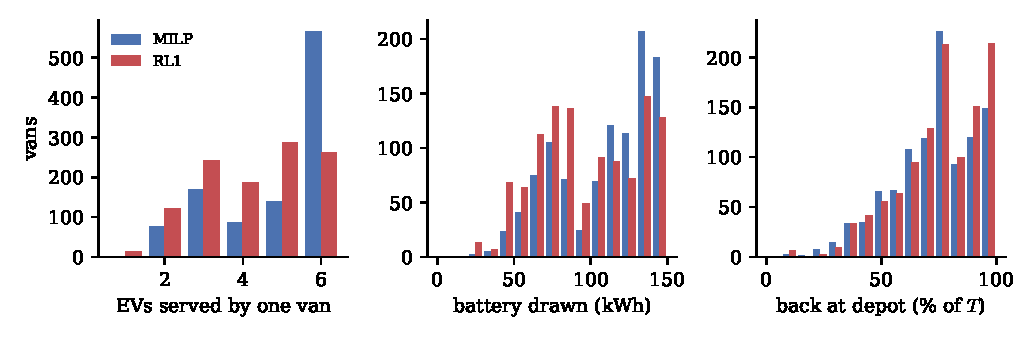
\includegraphics[width=\textwidth]{figures/r_vans.pdf}
\caption{EVs per van, battery drawn and return time; MILP and RL1.}
\label{fig:vans}
\end{figure}
\begin{itemize}
  \item RL1 sends out as many vans as the MILP (\VansPerPlanR{} per plan against \VansPerPlanM) but fills fewer seats: \VansFullR\pct{} of its vans are full (MILP \VansFullM\pct). \SeatsStrandedR\pct{} of its van seats go to stranded EVs (MILP \SeatsStrandedM\pct).
  \item The tightest van resource is time for \TightTimeR\pct{} of RL1 vans and seats for \TightSeatsR\pct{} (MILP: seats \TightSeatsM\pct, time \TightTimeM\pct). RL1 vans run their routes in a less time-efficient order and return later with free seats.
\end{itemize}

\inshort{RL1 pays for the same vans but uses them less: spare seats that the MILP fills with rich free-choice customers stay empty.}

%---------------------------------------------------------------------
\subsection{Money paid and perceived cost: equity}
\label{sec:equity}
\begin{figure}[H]
\centering
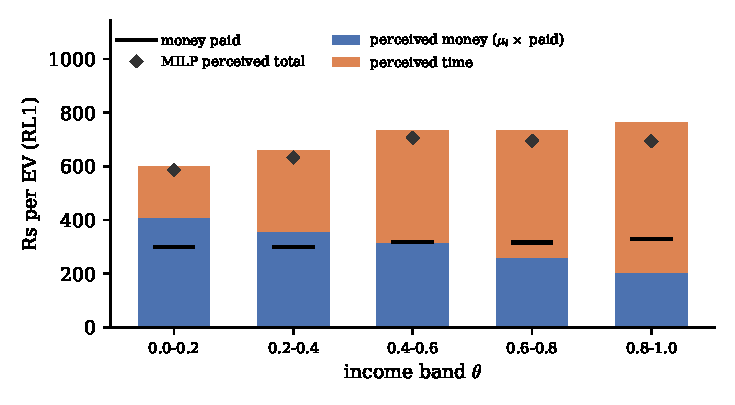
\includegraphics[width=0.7\textwidth]{figures/r_costs.pdf}
\caption{Money paid and perceived cost per EV by income band in RL1 plans (diamonds: MILP perceived total).}
\label{fig:costs}
\end{figure}
\begin{table}[H]
\centering\footnotesize
\caption{Shares of money paid and perceived cost by income band in RL1 plans.}
\label{tab:equity}
\begin{tabular}{@{}lrrrrrrr@{}}
\toprule
income $\theta$ & \shortstack[r]{share of\\EVs (\%)} & \shortstack[r]{share of\\money paid (\%)} & \shortstack[r]{share of\\perceived (\%)} & \shortstack[r]{perceived per\\Rs paid} & \shortstack[r]{RL1 perceived\\per EV (Rs)} & \shortstack[r]{MILP perceived\\per EV (Rs)} & \shortstack[r]{paid per\\kWh (Rs)} \\
\midrule
0.0--0.2 & 13.0 & 12.4 & 11.0 & 2.00 & 600 & 585 & 15.7 \\
0.2--0.4 & 20.9 & 20.1 & 19.7 & 2.21 & 661 & 633 & 15.7 \\
0.4--0.6 & 33.0 & 33.6 & 34.4 & 2.30 & 733 & 706 & 15.7 \\
0.6--0.8 & 23.5 & 23.8 & 24.5 & 2.32 & 734 & 696 & 16.1 \\
0.8--1.0 & 9.7 & 10.1 & 10.5 & 2.32 & 763 & 694 & 16.6 \\
\bottomrule
\end{tabular}

\end{table}
Perceived cost per rupee paid is \PerRsBotR{} in the poorest band and \PerRsTopR{} in the richest (MILP 1.94 and 1.88): RL1 plans leave the rich at the stations, so they pay less money but feel more time. The poor are affected little, because the MILP also left them at the stations.

\inshort{RL1's shortfall falls mostly on the rich, who miss vans and queue instead.}

%---------------------------------------------------------------------
\subsection{Sensitivity to the income distribution}
\label{sec:beta}
\begin{table}[H]
\centering\small
\caption{Expected van share of free-choice EVs under other income distributions (decile shares reweighted).}
\label{tab:beta}
\begin{tabular}{@{}lrrr@{}}
\toprule
income distribution & mean $\theta$ & \shortstack[r]{RL1 expected\\van share (\%)} & \shortstack[r]{MILP expected\\van share (\%)} \\
\midrule
Beta(1,1) uniform & 0.50 & 4.3 & 9.8 \\
Beta(2,2) (used) & 0.50 & 3.7 & 7.4 \\
Beta(2,5) mostly low income & 0.29 & 1.1 & 1.6 \\
Beta(5,2) mostly high income & 0.71 & 7.4 & 17.0 \\
Beta(0.5,0.5) polarised & 0.50 & 4.8 & 12.1 \\
\bottomrule
\end{tabular}

\end{table}
For every income distribution RL1's expected van share is about half the MILP's; a population leaning to high incomes would widen the absolute difference, because that is where RL1 departs from the MILP.

\inshort{The richer the population, the more RL1's missing vans cost.}

%---------------------------------------------------------------------
\subsection{Why RL1 behaves this way}
\label{sec:why}
\begin{itemize}
  \item \textbf{Step-wise reward.} Each action is charged its own increase of $Z$. A van's dispatch cost and its detour are paid at once, while the value of a spare seat (saving a rich customer a long station visit later) appears only through later actions. Learning such delayed credit is hard for REINFORCE with a per-instance baseline.
  \item \textbf{Warm start on the greedy rule.} Imitation copies a rule that places stranded EVs first and then takes the cheapest immediate option; the rule rarely adds free-choice customers to vans. REINFORCE improved on it (\BestValPct\pct{} on validation) but stopped early, still close to the rule's habits.
  \item \textbf{Append-only construction.} An EV can only be added at the end of a van route; the MILP can insert a rich customer between two stranded ones. Some good van routes cannot be built.
  \item \textbf{Generalisation.} Training uses generated instances; the test files differ in request patterns and clustering, especially at large $n$, where the gap is largest.
\end{itemize}
\textbf{What would close the gap:} imitate MILP plans instead of the greedy rule; train longer or with a smaller learning-rate decay (the $n=100$ curve was still noisy at the stop); give the decoder features that value a van's spare capacity; allow insertion into van routes; use RL1's plan as the MILP's warm start, which would also remove the 30 MILP instances without a plan.

\inshort{RL1 is close to the MILP because it learned the stations and the income threshold; it falls short because filling van seats with rich customers is a long-run effect that the step-wise reward and the greedy warm start hide.}

%---------------------------------------------------------------------
\subsection{Robustness and caveats}
\label{sec:robust}
\begin{itemize}
  \item \textbf{One training run, one seed.} Another seed or a longer run would give somewhat different numbers.
  \item \textbf{The MILP benchmark is not always optimal.} Gaps to time-limit plans are upper bounds of the true optimality gap; against proven optima the gap is \GapOptMean\pct.
  \item \textbf{Placeholder parameters.} As for the MILP, the size of every income effect depends on the placeholder values; RL1 would need retraining after recalibration.
  \item \textbf{Shadow prices are conditional} on each plan's decisions.
  \item \textbf{Hardware differs.} RL1 ran on a GPU, the MILP on 4 CPU threads per instance; the speed comparison is indicative.
\end{itemize}

%=====================================================================
\section{Summary of findings}
\begin{enumerate}
  \item RL1 gives valid plans in \NValidR{} instances (MILP \NValidM), including \RLonly{} the MILP could not solve, and never fails where the MILP succeeds.
  \item It costs \GapMean\pct{} more than the MILP on average (\GapOptMean\pct{} more than proven optima), beats the MILP in \RLbetter{} unfinished instances and the greedy rule in \GreedyBeat{} of \GreedyN.
  \item It solves an instance in \RLtime\,s, about \Speedup{} times faster than the MILP; training pays off after about \BreakEven{} instances.
  \item It agrees with the MILP's resource choice for \AgreeType\pct{} of free-choice EVs and reproduces the income threshold, but gives vans to rich customers about half as often.
  \item Its extra cost is waiting time: queues at peak are about twice the MILP's, and gun-minutes are scarce more often.
  \item Cost structure, elasticities and the zero value of patience limits and deadlines are the same as for the MILP.
  \item Imitating MILP plans, valuing spare van capacity and inserting into routes are the most promising improvements.
\end{enumerate}

\vspace{6pt}
{\footnotesize Generated from \texttt{../runs.csv}, \texttt{../plan.csv}, \texttt{../../model/train\_log.csv} and \texttt{../../../new\_results} by \texttt{compute\_duals\_rl.py} and \texttt{make\_rl\_report.py} in this folder.}

\end{document}
